\documentclass[12pt,ngerman,]{book}
\usepackage{lmodern}
\usepackage{amssymb,amsmath}
\usepackage{ifxetex,ifluatex}
\usepackage{fixltx2e} % provides \textsubscript
\ifnum 0\ifxetex 1\fi\ifluatex 1\fi=0 % if pdftex
  \usepackage[T1]{fontenc}
  \usepackage[utf8]{inputenc}
  \usepackage{eurosym}
\else % if luatex or xelatex
  \ifxetex
    \usepackage{mathspec}
  \else
    \usepackage{fontspec}
  \fi
  \defaultfontfeatures{Ligatures=TeX,Scale=MatchLowercase}
  \newcommand{\euro}{€}
\fi
% use upquote if available, for straight quotes in verbatim environments
\IfFileExists{upquote.sty}{\usepackage{upquote}}{}
% use microtype if available
\IfFileExists{microtype.sty}{%
\usepackage{microtype}
\UseMicrotypeSet[protrusion]{basicmath} % disable protrusion for tt fonts
}{}
\usepackage[margin=1in]{geometry}
\usepackage{hyperref}
\PassOptionsToPackage{usenames,dvipsnames}{color} % color is loaded by hyperref
\hypersetup{unicode=true,
            pdftitle={Praxis der Datenanalyse},
            pdfauthor={Sebastian Sauer. Mit Beiträgen von Oliver Gansser, Matthias Gehrke, Karsten Lübke und Norman Markgraf},
            colorlinks=true,
            linkcolor=Maroon,
            citecolor=Blue,
            urlcolor=Blue,
            breaklinks=true}
\urlstyle{same}  % don't use monospace font for urls
\ifnum 0\ifxetex 1\fi\ifluatex 1\fi=0 % if pdftex
  \usepackage[shorthands=off,main=ngerman]{babel}
\else
  \usepackage{polyglossia}
  \setmainlanguage[]{german}
\fi
\usepackage{color}
\usepackage{fancyvrb}
\newcommand{\VerbBar}{|}
\newcommand{\VERB}{\Verb[commandchars=\\\{\}]}
\DefineVerbatimEnvironment{Highlighting}{Verbatim}{commandchars=\\\{\}}
% Add ',fontsize=\small' for more characters per line
\usepackage{framed}
\definecolor{shadecolor}{RGB}{248,248,248}
\newenvironment{Shaded}{\begin{snugshade}}{\end{snugshade}}
\newcommand{\KeywordTok}[1]{\textcolor[rgb]{0.13,0.29,0.53}{\textbf{#1}}}
\newcommand{\DataTypeTok}[1]{\textcolor[rgb]{0.13,0.29,0.53}{#1}}
\newcommand{\DecValTok}[1]{\textcolor[rgb]{0.00,0.00,0.81}{#1}}
\newcommand{\BaseNTok}[1]{\textcolor[rgb]{0.00,0.00,0.81}{#1}}
\newcommand{\FloatTok}[1]{\textcolor[rgb]{0.00,0.00,0.81}{#1}}
\newcommand{\ConstantTok}[1]{\textcolor[rgb]{0.00,0.00,0.00}{#1}}
\newcommand{\CharTok}[1]{\textcolor[rgb]{0.31,0.60,0.02}{#1}}
\newcommand{\SpecialCharTok}[1]{\textcolor[rgb]{0.00,0.00,0.00}{#1}}
\newcommand{\StringTok}[1]{\textcolor[rgb]{0.31,0.60,0.02}{#1}}
\newcommand{\VerbatimStringTok}[1]{\textcolor[rgb]{0.31,0.60,0.02}{#1}}
\newcommand{\SpecialStringTok}[1]{\textcolor[rgb]{0.31,0.60,0.02}{#1}}
\newcommand{\ImportTok}[1]{#1}
\newcommand{\CommentTok}[1]{\textcolor[rgb]{0.56,0.35,0.01}{\textit{#1}}}
\newcommand{\DocumentationTok}[1]{\textcolor[rgb]{0.56,0.35,0.01}{\textbf{\textit{#1}}}}
\newcommand{\AnnotationTok}[1]{\textcolor[rgb]{0.56,0.35,0.01}{\textbf{\textit{#1}}}}
\newcommand{\CommentVarTok}[1]{\textcolor[rgb]{0.56,0.35,0.01}{\textbf{\textit{#1}}}}
\newcommand{\OtherTok}[1]{\textcolor[rgb]{0.56,0.35,0.01}{#1}}
\newcommand{\FunctionTok}[1]{\textcolor[rgb]{0.00,0.00,0.00}{#1}}
\newcommand{\VariableTok}[1]{\textcolor[rgb]{0.00,0.00,0.00}{#1}}
\newcommand{\ControlFlowTok}[1]{\textcolor[rgb]{0.13,0.29,0.53}{\textbf{#1}}}
\newcommand{\OperatorTok}[1]{\textcolor[rgb]{0.81,0.36,0.00}{\textbf{#1}}}
\newcommand{\BuiltInTok}[1]{#1}
\newcommand{\ExtensionTok}[1]{#1}
\newcommand{\PreprocessorTok}[1]{\textcolor[rgb]{0.56,0.35,0.01}{\textit{#1}}}
\newcommand{\AttributeTok}[1]{\textcolor[rgb]{0.77,0.63,0.00}{#1}}
\newcommand{\RegionMarkerTok}[1]{#1}
\newcommand{\InformationTok}[1]{\textcolor[rgb]{0.56,0.35,0.01}{\textbf{\textit{#1}}}}
\newcommand{\WarningTok}[1]{\textcolor[rgb]{0.56,0.35,0.01}{\textbf{\textit{#1}}}}
\newcommand{\AlertTok}[1]{\textcolor[rgb]{0.94,0.16,0.16}{#1}}
\newcommand{\ErrorTok}[1]{\textcolor[rgb]{0.64,0.00,0.00}{\textbf{#1}}}
\newcommand{\NormalTok}[1]{#1}
\usepackage{longtable,booktabs}
\usepackage{graphicx,grffile}
\makeatletter
\def\maxwidth{\ifdim\Gin@nat@width>\linewidth\linewidth\else\Gin@nat@width\fi}
\def\maxheight{\ifdim\Gin@nat@height>\textheight\textheight\else\Gin@nat@height\fi}
\makeatother
% Scale images if necessary, so that they will not overflow the page
% margins by default, and it is still possible to overwrite the defaults
% using explicit options in \includegraphics[width, height, ...]{}
\setkeys{Gin}{width=\maxwidth,height=\maxheight,keepaspectratio}
\usepackage[normalem]{ulem}
% avoid problems with \sout in headers with hyperref:
\pdfstringdefDisableCommands{\renewcommand{\sout}{}}
\IfFileExists{parskip.sty}{%
\usepackage{parskip}
}{% else
\setlength{\parindent}{0pt}
\setlength{\parskip}{6pt plus 2pt minus 1pt}
}
\setlength{\emergencystretch}{3em}  % prevent overfull lines
\providecommand{\tightlist}{%
  \setlength{\itemsep}{0pt}\setlength{\parskip}{0pt}}
\setcounter{secnumdepth}{5}
% Redefines (sub)paragraphs to behave more like sections
\ifx\paragraph\undefined\else
\let\oldparagraph\paragraph
\renewcommand{\paragraph}[1]{\oldparagraph{#1}\mbox{}}
\fi
\ifx\subparagraph\undefined\else
\let\oldsubparagraph\subparagraph
\renewcommand{\subparagraph}[1]{\oldsubparagraph{#1}\mbox{}}
\fi

%%% Use protect on footnotes to avoid problems with footnotes in titles
\let\rmarkdownfootnote\footnote%
\def\footnote{\protect\rmarkdownfootnote}

%%% Change title format to be more compact
\usepackage{titling}

% Create subtitle command for use in maketitle
\newcommand{\subtitle}[1]{
  \posttitle{
    \begin{center}\large#1\end{center}
    }
}

\setlength{\droptitle}{-2em}
  \title{Praxis der Datenanalyse}
  \pretitle{\vspace{\droptitle}\centering\huge}
  \posttitle{\par}
\subtitle{Skript zum Modul}
  \author{Sebastian Sauer. Mit Beiträgen von Oliver Gansser, Matthias Gehrke,
Karsten Lübke und Norman Markgraf}
  \preauthor{\centering\large\emph}
  \postauthor{\par}
  \predate{\centering\large\emph}
  \postdate{\par}
  \date{06 July, 2017}

\usepackage{booktabs}
\usepackage{longtable}
\usepackage[bf,singlelinecheck=off]{caption}

%ses:
\pagestyle{headings}

%\setmainfont[UprightFeatures={SmallCapsFont=AlegreyaSC-Regular}]{Alegreya}

\usepackage{framed,color}
\definecolor{shadecolor}{RGB}{248,248,248}

\renewcommand{\textfraction}{0.05}
\renewcommand{\topfraction}{0.8}
\renewcommand{\bottomfraction}{0.8}
\renewcommand{\floatpagefraction}{0.75}

%\renewenvironment{quote}{\begin{VF}}{\end{VF}}
\let\oldhref\href
\renewcommand{\href}[2]{#2\footnote{\url{#1}}}

\ifxetex
  \usepackage{letltxmacro}
  \setlength{\XeTeXLinkMargin}{1pt}
  \LetLtxMacro\SavedIncludeGraphics\includegraphics
  \def\includegraphics#1#{% #1 catches optional stuff (star/opt. arg.)
    \IncludeGraphicsAux{#1}%
  }%
  \newcommand*{\IncludeGraphicsAux}[2]{%
    \XeTeXLinkBox{%
      \SavedIncludeGraphics#1{#2}%
    }%
  }%
\fi

% Hier müsste noch das Chapter mit rein! Sonst gibt es Das nicht in der Ausgabe!
% Daher habe ich das auskommentiert! (NM)
%\renewcommand{\thesection}{\arabic{section}}  % ses


\makeatletter
\newenvironment{kframe}{%
\medskip{}
\setlength{\fboxsep}{.8em}
 \def\at@end@of@kframe{}%
 \ifinner\ifhmode%
  \def\at@end@of@kframe{\end{minipage}}%
  \begin{minipage}{\columnwidth}%
 \fi\fi%
 \def\FrameCommand##1{\hskip\@totalleftmargin \hskip-\fboxsep
 \colorbox{shadecolor}{##1}\hskip-\fboxsep
     % There is no \\@totalrightmargin, so:
     \hskip-\linewidth \hskip-\@totalleftmargin \hskip\columnwidth}%
 \MakeFramed {\advance\hsize-\width
   \@totalleftmargin\z@ \linewidth\hsize
   \@setminipage}}%
 {\par\unskip\endMakeFramed%
 \at@end@of@kframe}
\makeatother

\renewenvironment{Shaded}{\begin{kframe}}{\end{kframe}}

\newenvironment{rmdblock}[1]
  {
  \begin{itemize}
  \renewcommand{\labelitemi}{
    \raisebox{-.7\height}[0pt][0pt]{
      {\setkeys{Gin}{width=3em,keepaspectratio}\includegraphics{images/icons/#1}}
    }
  }
  \setlength{\fboxsep}{1em}
  \begin{kframe}
  \item
  }
  {
  \end{kframe}
  \end{itemize}
  }
\newenvironment{rmdnote}
  {\begin{rmdblock}{note}}
  {\end{rmdblock}}
\newenvironment{rmdcaution}
  {\begin{rmdblock}{caution}}
  {\end{rmdblock}}
\newenvironment{rmdimportant}
  {\begin{rmdblock}{important}}
  {\end{rmdblock}}
\newenvironment{rmdtip}
  {\begin{rmdblock}{tip}}
  {\end{rmdblock}}
\newenvironment{rmdwarning}
  {\begin{rmdblock}{warning}}
  {\end{rmdblock}}
\newenvironment{rmdpseudocode}
  {\begin{rmdblock}{pseudocode}}
  {\end{rmdblock}}
\newenvironment{rmdexercises}
  {\begin{rmdblock}{exercises}}
  {\end{rmdblock}}
\newenvironment{rmdlove}
  {\begin{rmdblock}{love}}
  {\end{rmdblock}}

\usepackage{makeidx}  % ses
\makeindex  % ses

\urlstyle{tt}

\usepackage{amsthm}
\makeatletter
\def\thm@space@setup{%
  \thm@preskip=8pt plus 2pt minus 4pt
  \thm@postskip=\thm@preskip
}


%NM:
\def\@makechapterhead#1{%
  \vspace*{50\p@}%
  {\parindent \z@ \raggedright \normalfont
  \ifnum \c@secnumdepth >\m@ne
    \if@mainmatter
        \huge\scshape\bfseries\scshape \@chapapp\space \thechapter
        \par\nobreak
        \vskip 20\p@
    \fi
  \fi
  \interlinepenalty\@M
  \Huge \scshape\bfseries\scshape #1\par\nobreak
  \vskip 40\p@
}}

\makeatother


% NM: Zu einem frontmatter gehört auch ein mainmatter, appendix und backmatter! ;-) - Habe ich daher mal eingefügt!
\frontmatter

\usepackage{amsthm}
\newtheorem{theorem}{Theorem}[chapter]
\newtheorem{lemma}{Lemma}[chapter]
\theoremstyle{definition}
\newtheorem{definition}{Definition}[chapter]
\newtheorem{corollary}{Corollary}[chapter]
\newtheorem{proposition}{Proposition}[chapter]
\theoremstyle{definition}
\newtheorem{example}{Example}[chapter]
\theoremstyle{remark}
\newtheorem*{remark}{Remark}
\let\BeginKnitrBlock\begin \let\EndKnitrBlock\end
\begin{document}
\maketitle

{
\hypersetup{linkcolor=black}
\setcounter{tocdepth}{2}
\tableofcontents
}
\listoftables
\listoffigures
\chapter{Placeholder}\label{placeholder}

\chapter{Organisatorisches}\label{organisatorisches}

\mainmatter

\setcounter{chapter}{0} \part{Grundlagen}

\chapter{Rahmen}\label{Rahmen}

\begin{center}
\includegraphics[width=0.3\linewidth]{images/FOM} \end{center}

\begin{center}
\includegraphics[width=0.1\linewidth]{images/licence} \end{center}

\BeginKnitrBlock{rmdcaution}
Lernziele:

\begin{itemize}
\tightlist
\item
  Einen Überblick über die fünf wesentliche Schritte der Datenanalyse
  gewinnen.
\item
  R und RStudio installieren können.
\item
  Einige häufige technische Probleme zu lösen wissen.
\item
  R-Pakete installieren können.
\item
  Einige grundlegende R-Funktionalitäten verstehen.
\item
  Auf die Frage ``Was ist Statistik?'' eine Antwort geben können.
\end{itemize}
\EndKnitrBlock{rmdcaution}

In diesem Skript geht es um die Praxis der Datenanalyse. Mit Rahmen ist
das ``Drumherum'' oder der Kontext der eigentlichen Datenanalyse
gemeint. Dazu gehören einige praktische Vorbereitungen und ein paar
Überlegungen. Zum Beispiel brauchen wir einen Überblick über das Thema.
Voilà (Abb. \ref{fig:fig-prozess}):

\begin{figure}

{\centering 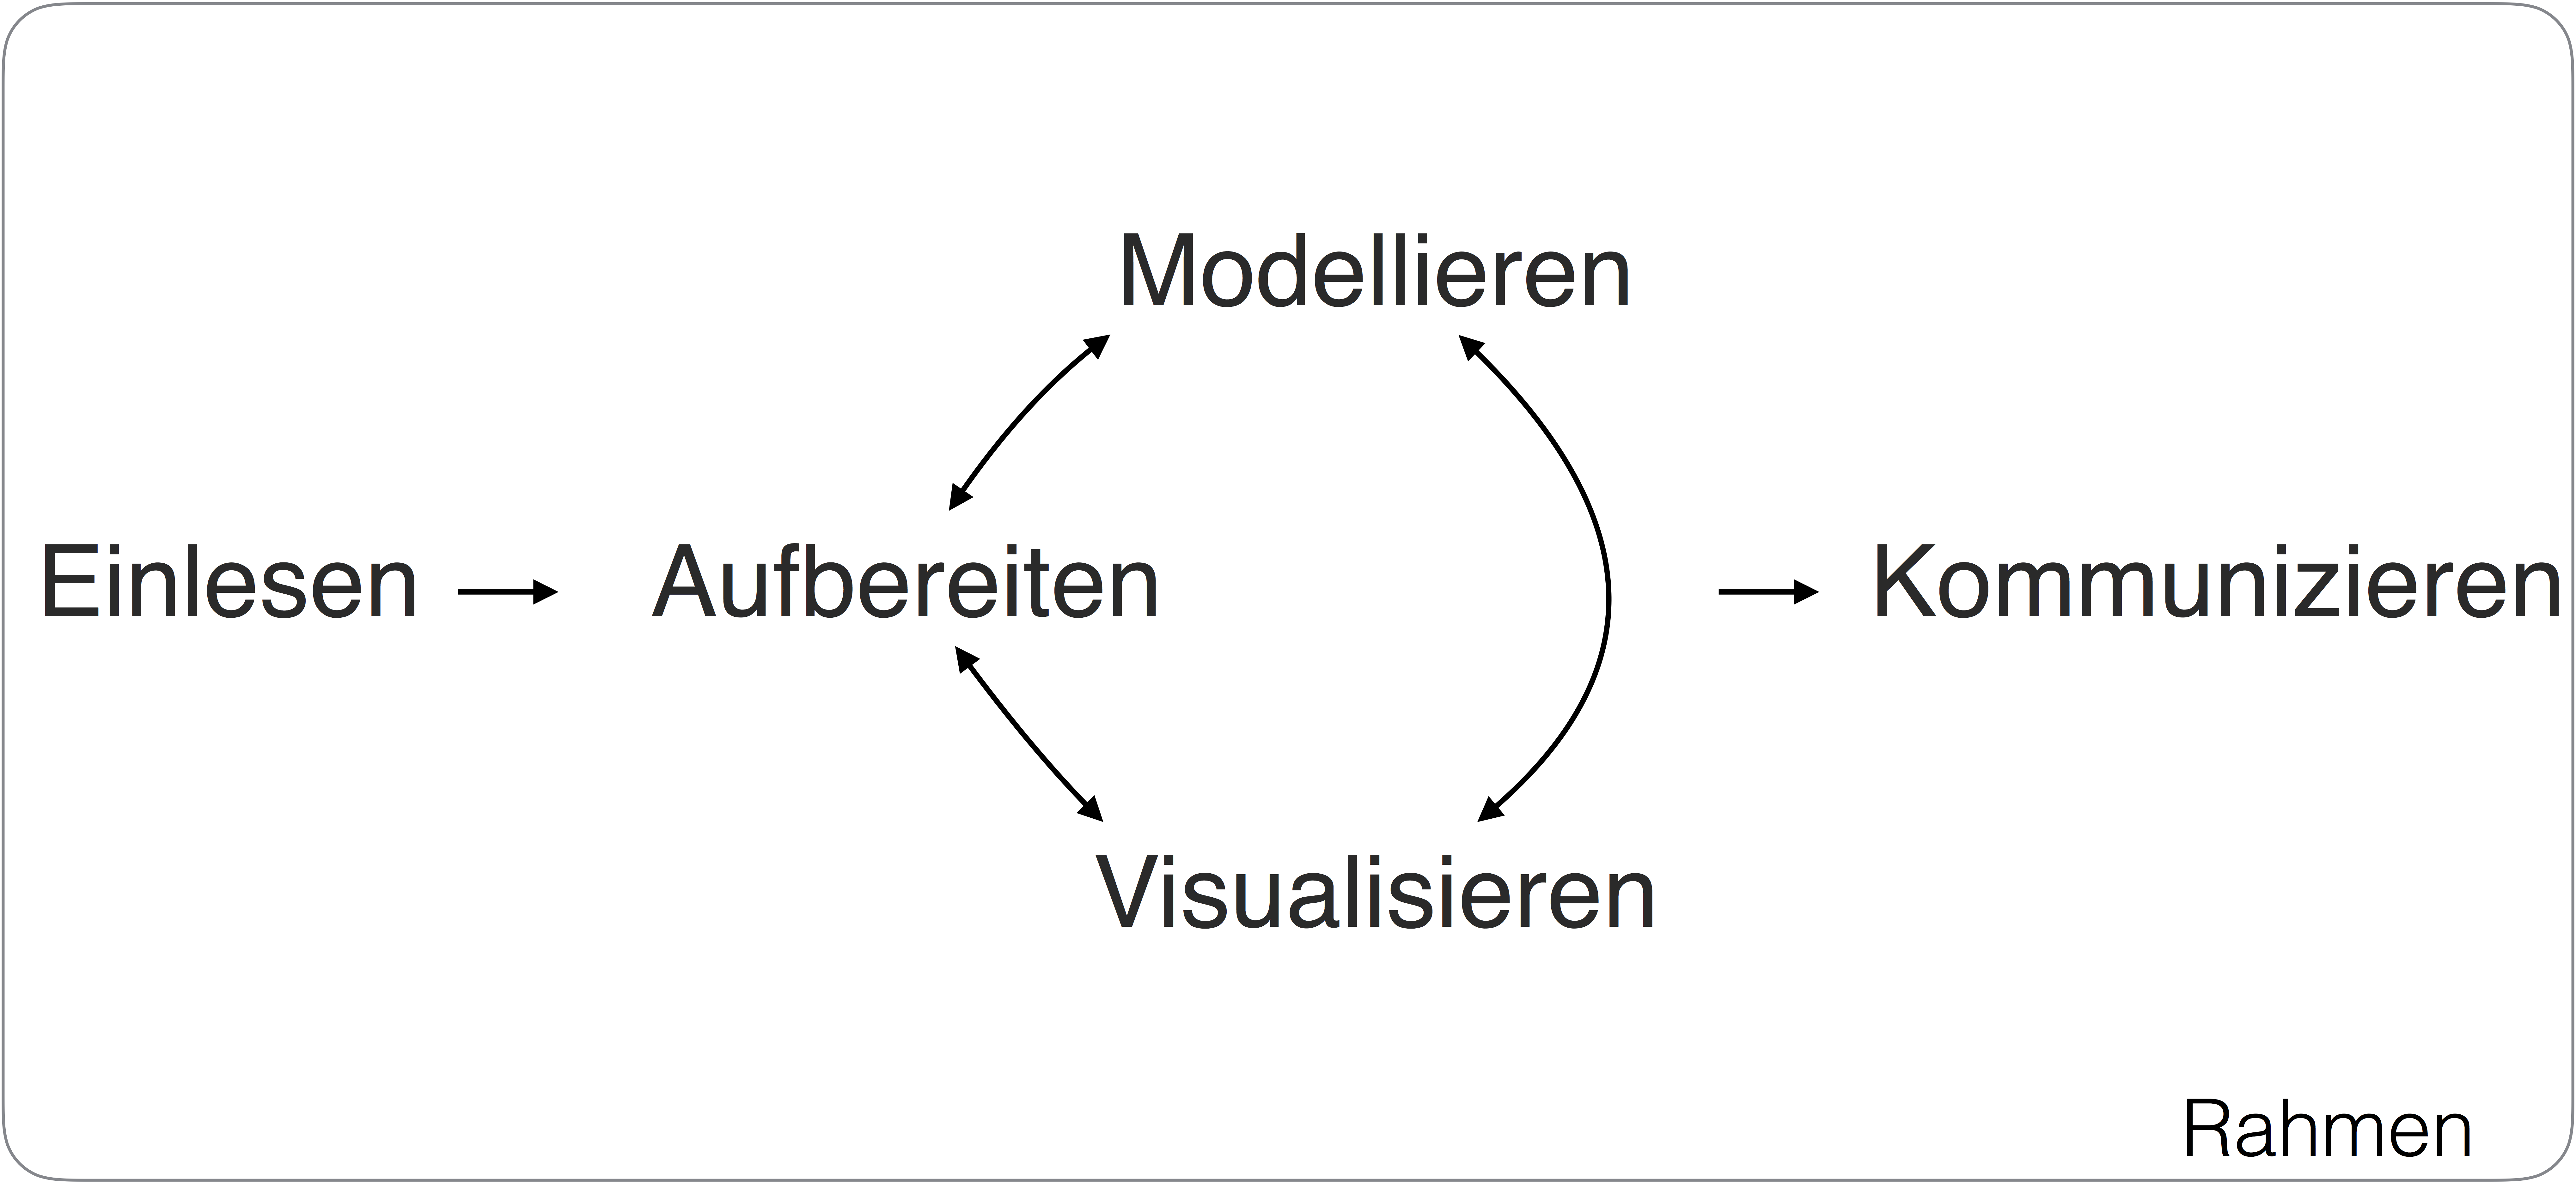
\includegraphics[width=0.7\linewidth]{images/Rahmen/Prozess_Datenanalyse} 

}

\caption{Der Prozess der Datenanalyse}\label{fig:fig-prozess}
\end{figure}

Datenanalyse, praktisch betrachtet, kann man in fünf Schritte einteilen
(Wickham und Grolemund \protect\hyperlink{ref-r4ds}{2016}). Zuerst muss
man die Daten \emph{einlesen}, die Daten also in R (oder einer anderen
Software) verfügbar machen (laden). Fügen wir hinzu: In \emph{schöner
Form} verfügbar machen; man nennt dies auch \emph{tidy data} (hört sich
cooler an). Sobald die Daten in geeigneter Form in R geladen sind, folgt
das \emph{Aufbereiten}. Das beinhaltet Zusammenfassen, Umformen oder
Anreichern je nach Bedarf. Ein nächster wesentlicher Schritt ist das
\emph{Visualisieren} der Daten. Ein Bild sagt bekanntlich mehr als viele
Worte. Schließlich folgt das \emph{Modellieren} oder das Hypothesen
prüfen: Man überlegt sich, wie sich die Daten erklären lassen könnten.
Zu beachten ist, dass diese drei Schritte - Aufbereiten, Visualisieren,
Modellieren - keine starre Abfolge sind, sondern eher ein munteres
Hin-und-Her-Springen, ein aufbauendes Abwechseln. Der letzte Schritt ist
das \emph{Kommunizieren} der Ergebnisse der Analyse - nicht der Daten.
Niemand ist an Zahlenwüsten interessiert; es gilt, spannende Einblicke
zu vermitteln.

Der Prozess der Datenanalyse vollzieht sich nicht im luftleeren Raum,
sondern ist in einem \emph{Rahmen} eingebettet. Dieser beinhaltet
praktische Aspekte - wie Software, Datensätze - und grundsätzliche
Überlegungen - wie Ziele und Grundannahmen.

\section{Software installieren}\label{software-installieren}

Als Haupt-Analysewerkzeug nutzen wir R; daneben wird uns die sog.
``Entwicklungsumgebung'' RStudio einiges an komfortabler Funktionalität
bescheren. Eine Reihe von R-Paketen (``Packages''; d.h. Erweiterungen)
werden wir auch nutzen. R ist eine recht alte Sprache; viele Neuerungen
finden in Paketen Niederschlag, da der ``harte Kern'' von R lieber nicht
so stark geändert wird. Stellen Sie sich vor: Seit 29 Jahren nutzen Sie
eine Befehl, der Ihnen einen Mittelwert ausrechnet, sagen wir die
mittlere Anzahl von Tassen Kaffee am Tag. Und auf einmal wird der
Mittelwert anders berechnet?! Eine Welt stürzt ein! Naja, vielleicht
nicht ganz so tragisch in dem Beispiel, aber grundsätzlich sind
Änderungen in viel benutzen Befehlen potenziell problematisch. Das ist
wohl ein Grund, warum sich am ``R-Kern'' nicht so viel ändert. Die
Innovationen in R passieren in den Paketen. Und es gibt viele davon; als
ich diese Zeilen schreibe, sind es fast schon 10.000! Genauer: 9937 nach
dieser Quelle: \url{https://cran.r-project.org/web/packages/}. Übrigens
können R-Pakete auch Daten enthalten.

\subsection{R und RStudio
installieren}\label{r-und-rstudio-installieren}


\includegraphics[width=0.10000\textwidth]{images/Rahmen/Rlogo.png}

\includegraphics[width=0.20000\textwidth]{images/Rahmen/rstudiologo.png}

Sie können R unter \url{https://cran.r-project.org} herunterladen und
installieren (für Windows, Mac oder Linux). RStudio finden Sie auf der
gleichnamigen Homepage: \url{https://www.rstudio.com}; laden Sie die
``Desktop-Version'' für Ihr Betriebssystem herunter.

RStudio ist ``nur'' eine Oberfläche (``GUI'') für R, mit einer R von
praktischen Zusatzfunktionen. Die eigentlich Arbeit verrichtet das
``normale'' R, welches automatisch gestartet wird, wenn Sie RStudio
starten (sofern R installiert ist).

Die Oberfläche von RStudio sieht (unter allen Betriebssystemen etwa
gleich) so aus wie in Abbildung \ref{fig:rstudio-screenshot}
dargestellt.

\begin{figure}

{\centering 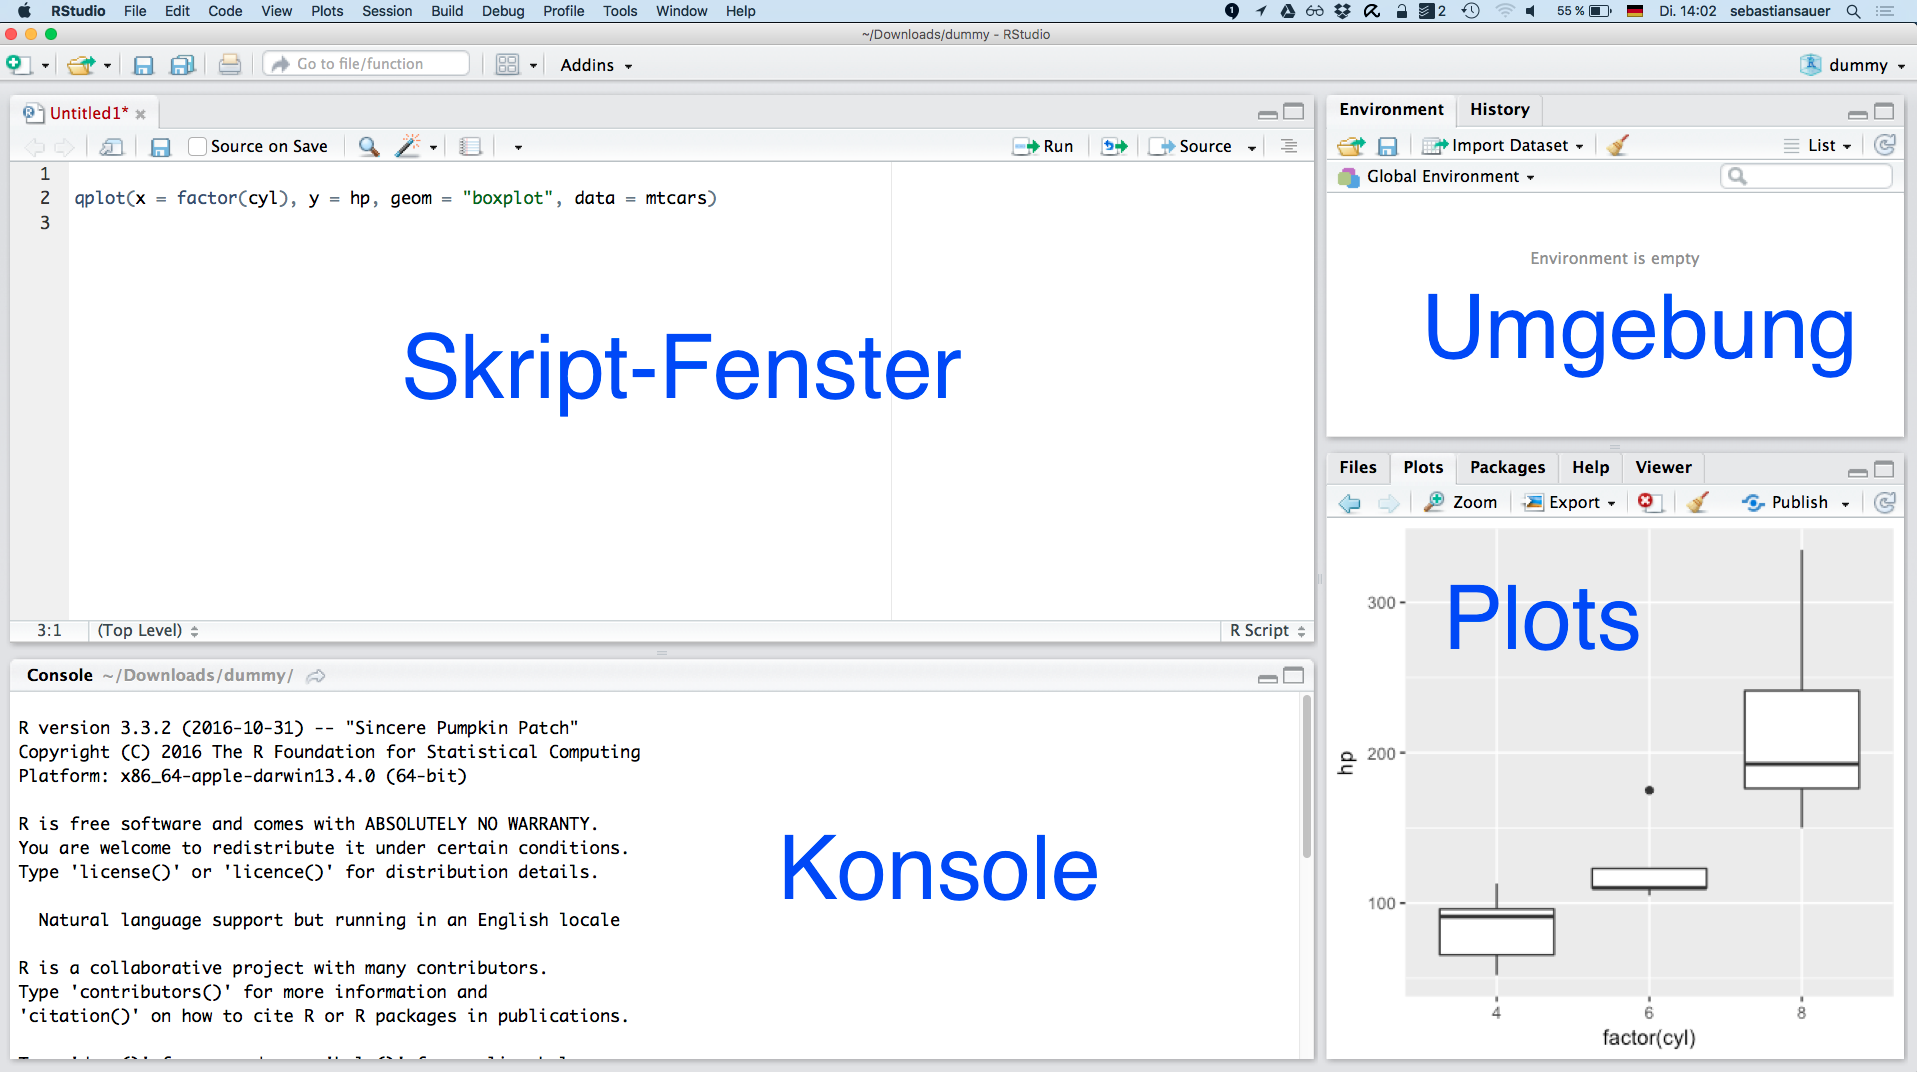
\includegraphics[width=0.7\linewidth]{images/Rahmen/RStudio-Screenshot} 

}

\caption{RStudio}\label{fig:rstudio-screenshot}
\end{figure}

Das \emph{Skript-Fenster}\index{Skript-Fenster} ähnelt einem normalem
Text-Editor; praktischerweise finden Sie aber einen Button ``run'', der
die aktuelle Zeile oder die Auswahl ``abschickt'', d.h. in die Konsole
gibt, wo die Syntax ausgeführt wird. Wenn Sie ein Skript-Fenster öffnen
möchten, so können Sie das Icon

\includegraphics{images/Rahmen/new_script.png} klicken (Alternativ:
Ctrl-Shift-N oder File \textgreater{} New File \textgreater{} R Script).

Aus dem Fenster der \emph{Konsole}\index{Konsole} spricht R zu uns bzw.
wir mit R. Wird ein Befehl\index{Funktion} (synonym:
\emph{Funktion}\index{Funktion}) hier eingegeben, so führt R ihn aus. Es
ist aber viel praktischer, Befehle in das Skript-Fenster einzugeben, als
in die Konsole. Behalten Sie dieses Fenster im Blick, wenn Sie Antwort
von R erwarten.

Im Fenster \emph{Umgebung}\index{Umgebung} (engl. ``environment'') zeigt
R, welche Variablen (Objekte) vorhanden sind. Stellen Sie sich die
Umgebung wie einen Karpfenteich vor, in dem die Datensätze und andere
Objekte herumschwimmen. Was nicht in der Umgebung angezeigt wird,
existiert nicht für R.

Im Fenster rechts unten werden mehrere Informationen bereit gestellt,
z.B. werden Diagramme (Plots) dort ausgegeben. Klicken Sie mal die
anderen Reiter im Fenster rechts unten durch.

Wer Shortcuts mag, wird in RStudio überschwänglich beschenkt; der
Shortcut für die Shortcuts ist \texttt{Shift-Alt-K}.

Wenn Sie RStudio starten, startet R automatisch auch. Starten Sie daher,
wenn Sie RStudio gestartet haben, \emph{nicht} noch extra R. Damit
hätten Sie sonst zwei Instanzen von R laufen, was zu Verwirrungen (bei R
und beim Nutzer) führen kann.

\subsection{Pakete}\label{pakete}

Ein Großteil der Neuentwicklungen bei R passiert in sog. `Paketen'
(engl. \emph{packages}), das sind Erweiterungen für R. Jeder, der sich
berufen fühlt, kann ein R-Paket schreiben und es zum `R-Appstore'
(\href{https://cran.r-project.org/}{CRAN}) hochladen. Von dort kann es
dann frei (frei wie in Bier) heruntergeladen werden.

Am einfachsten installiert man R-Pakete in RStudio über den Button
``Install'' im Reiter ``Packages'' (s. Abb.
\ref{fig:fig-install-packages}).

\begin{figure}

{\centering 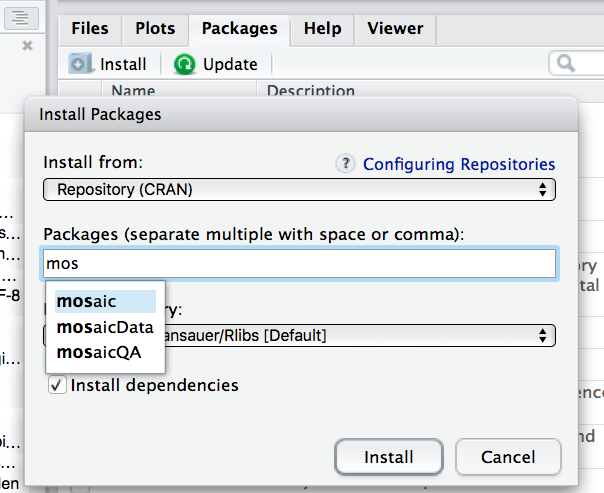
\includegraphics[width=0.7\linewidth]{images/Rahmen/install_packages} 

}

\caption{So installiert man Pakete in RStudio}\label{fig:fig-install-packages}
\end{figure}

Ein R-Paket, welches wir gleich benötigen, heißt \texttt{devtools}.
Bitte installieren Sie es schon einmal (sofern noch nicht geschehen).
Sie können auch folgenden Befehl verwenden, um Pakete zu installieren.

\begin{Shaded}
\begin{Highlighting}[]
\KeywordTok{install.packages}\NormalTok{(}\StringTok{"devtools"}\NormalTok{, }\DataTypeTok{dependencies =} \OtherTok{TRUE}\NormalTok{) }
\end{Highlighting}
\end{Shaded}

Aber einfacher geht es über die RStudio-Oberfläche.

Alle Pakete außer \texttt{devtools}, die wir hier benötigen, können über
das R-Paket \texttt{prada} installiert werden. Sie müssen also nur noch
das Paket \texttt{prada}installieren. Mit dem Befehl
\texttt{install\_prada\_pckgs} (aus dem Paket \texttt{prada}) werdenn
dann ggf. eine Reihe weiterer Pakete installiert. Allerdings wohnt
\texttt{prada} nicht im R-Appstore (CRAN), sondern bei
\href{www.github.com}{Github}\footnote{einer Online-Plattform, auf der
  man Dateien bereistellen und ihre Veränderungen nachverfolgen kann}.
Um Pakete von Github zu installieren, nutzen wir diesen Befehl (Sie
müssen natürlich online sein):

\begin{Shaded}
\begin{Highlighting}[]
\NormalTok{devtools}\OperatorTok{::}\KeywordTok{install_github}\NormalTok{(}\StringTok{"sebastiansauer/prada"}\NormalTok{)}
\KeywordTok{library}\NormalTok{(prada)}
\end{Highlighting}
\end{Shaded}

Sofern Sie online sind, sollte das Paket \texttt{prada} jetzt
installiert sein. Installieren Sie jetzt alle Pakete, die für diesen
Kurs benötigt werden mit dem Befehl \texttt{install\_prada\_pckgs()}.

\BeginKnitrBlock{rmdcaution}
Beim Installieren von R-Paketen könnten Sie gefragt werden, welchen
``Mirror'' Sie verwenden möchten. Das hat folgenden Hintergrund:
R-Pakete sind in einer Art ``App-Store'', mit Namen CRAN (Comprehense R
Archive Network) gespeichert. Damit nicht ein armer, kleiner Server
überlastet wird, wenn alle Studis dieser Welt just gerade beschließen,
ein Paket herunterzuladen, gibt es viele Kopien dieses Servers - seine
Spiegelbilder (engl. ``mirrors''). Suchen Sie sich einfach einen aus,
der in der Nähe ist.

Bei der Installation von Paketen mit
\texttt{install.packages("name\_des\_pakets")} sollte stets der
Parameter \texttt{dependencies\ =\ TRUE} angefügt werden. Also
\texttt{install.packages("name\_des\_pakets",\ dependencies\ =\ TRUE)}.
Hintergrund ist: Falls das zu installierende Paket seinerseits Pakete
benötigt, die noch nicht installiert sind (gut möglich), dann werden
diese sog. ``dependencies'' gleich mitinstalliert (wenn Sie
\texttt{dependencies\ =\ TRUE} setzen).
\EndKnitrBlock{rmdcaution}

Nicht vergessen: Installieren muss man eine Software \emph{nur einmal};
\emph{starten} (laden) muss man die R-Pakete jedes Mal, wenn man sie
vorher geschlossen hat und wieder nutzen möchte.

\begin{quote}
Wenn Sie R bzw. RStudio schließen, werden alle Pakete ebenfalls
geschlossen. Sie müssen die benötigten Pakete beim erneuten Öffnen von
RStudio wieder starten.
\end{quote}

\begin{Shaded}
\begin{Highlighting}[]
\KeywordTok{library}\NormalTok{(dplyr) }
\end{Highlighting}
\end{Shaded}

Der Befehl bedeutet sinngemäß: ``Hey R, geh in die Bücherei (library)
und hole das Buch (package) dplyr!''.

\BeginKnitrBlock{rmdcaution}
Wann benutzt man bei R Anführungszeichen? Das ist etwas verwirrend im
Detail, aber die Grundegel lautet: wenn man Text anspricht. Im Beispiel
oben ``library(dplyr)'' ist ``dplyr'' hier erst mal für R nichts
Bekanntes, weil noch nicht geladen. Demnach müssten \emph{eigentlich}
Anführungsstriche stehen. Allerdings meinte ein Programmierer, dass es
doch so bequemer ist. Hat er Recht. Aber bedenken Sie, dass es sich um
die Ausnahme einer Regel handelt. Sie können also auch schreiben:
library(``dplyr'') oder library(`dplyr'); beides geht.
\EndKnitrBlock{rmdcaution}

\subsection{Hilfe! R startet nicht!}\label{hilfe-r-startet-nicht}

\begin{quote}
Manntje, Manntje, Timpe Te,\\
Buttje, Buttje inne See,\\
myne Fru de Ilsebill\\
will nich so, as ik wol will.
\end{quote}

\emph{Gebrüder Grimm, Märchen vom Fischer und seiner Frau\footnote{\url{https://de.wikipedia.org/wiki/Vom_Fischer_und_seiner_Frau}}}

Ihr R startet nicht oder nicht richtig? Die drei wichtigsten Heilmittel
sind:

\begin{enumerate}
\def\labelenumi{\arabic{enumi}.}
\tightlist
\item
  Schließen Sie die Augen für eine Minute. Denken Sie an etwas Schönes
  und was Rs Problem sein könnte.
\item
  Schalten Sie den Rechner aus und probieren Sie es morgen noch einmal.
\item
  Googeln.
\end{enumerate}

Sorry für die schnoddrigen Tipps. Aber: Es passiert allzu leicht, dass
man \emph{Fehler} wie diese macht:

\BeginKnitrBlock{rmdcaution}
OH NO:

\begin{itemize}
\item
  install.packages(dplyr)
\item
  install.packages(``dliar'')
\item
  install.packages(``derpyler'')
\item
  install.packages(``dplyr'') \# dependencies vergessen
\item
  Keine Internet-Verbindung
\item
  library(dplyr) \# ohne vorher zu installieren
\end{itemize}
\EndKnitrBlock{rmdcaution}

Wenn R oder RStudio dann immer noch nicht starten oder nicht richtig
laufen, probieren Sie dieses:

\begin{itemize}
\item
  Sehen Sie eine Fehlermeldung, die von einem fehlenden Paket spricht
  (z.B. ``Package `Rcpp' not available'') oder davon spricht, dass ein
  Paket nicht installiert werden konnte (z.B. ``Package `Rcpp' could not
  be installed'' oder ``es gibt kein Paket namens `Rcpp'\,'' oder
  ``unable to move temporary installation XXX to YYY''), dann tun Sie
  folgendes:
\item
  Schließen Sie R und starten Sie es neu.
\item
  Installieren Sie das oder die angesprochenen Pakete\footnote{\texttt{install.packages("name\_des\_pakets",\ dependencies\ =\ TRUE)}
    oder mit dem entsprechenden Klick in RStudio}.
\item
  Starten Sie das entsprechende Paket mit
  \texttt{library(name\_des\_pakets)}.
\item
  Gerade bei Windows 10 scheinen die Schreibrechte für R (und damit
  RStudio oder RCommander) eingeschränkt zu sein. Ohne Schreibrechte
  kann R aber nicht die Pakete (``packages'') installieren, die Sie für
  bestimmte R-Funktionen benötigen. Daher schließen Sie R bzw. RStudio
  und suchen Sie das Icon von R oder wenn Sie RStudio verwenden von
  RStudio. Rechtsklicken Sie das Icon und wählen Sie ``als Administrator
  ausführen''. Damit geben Sie dem Programm Schreibrechte. Jetzt können
  Sie etwaige fehlende Pakete installieren.
\item
  Ein weiterer Grund, warum R bzw. RStudio die Schreibrechte verwehrt
  werden könnten (und damit die Installation von Paketen), ist ein
  Virenscanner. Der Virenscanner sagt, nicht ganz zu Unrecht: ``Moment,
  einfach hier Software zu installieren, das geht nicht, zu
  gefährlich''. Grundsätzlich gut, in diesem Fall unnötig. Schließen Sie
  R/RStudio und schalten Sie dann den Virenscanner \emph{komplett} (!)
  aus. Öffnen Sie dann R/RStudio wieder und versuchen Sie fehlende
  Pakete zu installieren.
\end{itemize}

\BeginKnitrBlock{rmdcaution}
Verwenden Sie möglichst die neueste Version von R, RStudio und Ihres
Betriebssystems. Ältere Versionen führen u.U. zu Problemen; je älter,
desto Problem\ldots{} Updaten Sie Ihre Packages regelmäßig z.B. mit
\texttt{update.packages()} oder dem Button ``Update'' bei RStudio
(Reiter \texttt{Packages}).
\EndKnitrBlock{rmdcaution}

\subsection{Vertiefung: Zuordnung von Paketen zu
Befehlen}\label{funs-pckgs}

\emph{Woher weiß man, welche Befehle (oder auch Daten) in einem Paket
enthalten sind?}

Eine einfache Möglichkeit ist es, beim Reiter `Pakete' auf den Namen
eines der installierten Pakete zu klicken. Daraufhin öffnet sich die
Dokumentation des Pakets und man sieht dort alle Befehle und Daten
aufgeführt (s. Abbildung \ref{fig:pakete-hilfe}). Übrigens sehen Sie
dort auch die Version eines Pakets (vielleicht sagt jemand mal zu Ihnen,
``Sie sind ja outdated'', dann schauen Sie mal auf die die
Paket-Versionen).

\begin{figure}

{\centering 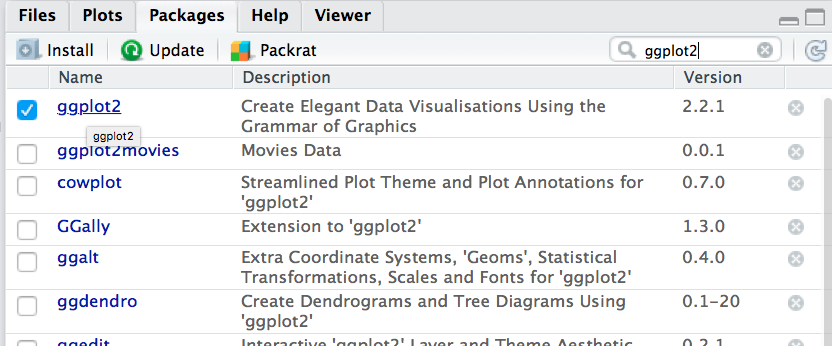
\includegraphics[width=0.5\linewidth]{images/Rahmen/hilfe_pakete} 

}

\caption{Hier werden Sie geholfen: Die Dokumentation der R-Pakete}\label{fig:pakete-hilfe}
\end{figure}

Für geladenen Pakete kann man auch den Befehl \texttt{help} nutzen, z.B.
\texttt{help(ggplot2)}.

\emph{Und umgekehrt, woher weiß ich, in welchem Paket ein Befehl
`wohnt'?}

Probieren Sie den Befehl \texttt{help.search("qplot")}, wenn Sie wissen
möchten, in welchem Paket \texttt{qplot} zuhause ist.
\texttt{help.search} sucht alle Hilfeseiten von \emph{installierten}
Paketen, in der der Suchbegriff irgendwie vorkommt. Um das Paket eines
\emph{geladenen} Befehl zu finden, hilft der Befehl \texttt{find}:
\texttt{find("qplot")}.

Sie können auch den Befehl \texttt{find\_fun}s aus dem Paket
\texttt{prada} nutzen:

\begin{Shaded}
\begin{Highlighting}[]
\NormalTok{prada}\OperatorTok{::}\KeywordTok{find_funs}\NormalTok{(}\StringTok{"select"}\NormalTok{)}
\CommentTok{#> # A tibble: 5 x 3}
\CommentTok{#>   package_name builtin_pckage loaded}
\CommentTok{#>          <chr>          <lgl>  <lgl>}
\CommentTok{#> 1        dplyr          FALSE  FALSE}
\CommentTok{#> 2         MASS           TRUE  FALSE}
\CommentTok{#> 3       plotly          FALSE  FALSE}
\CommentTok{#> 4       raster          FALSE  FALSE}
\CommentTok{#> 5         VGAM          FALSE  FALSE}
\end{Highlighting}
\end{Shaded}

In diesem Skript sind am Ende jedes Kapitels die jeweils besprochenen
(neuen) Befehle aufgeführt - inklusive ihres Paketes. Falls bei einem
Befehl kein Paket angegeben ist, heißt das, dass der Befehl im
`Standard-R' wohnt - Sie müssen kein weiteres Paket laden\footnote{Eine
  Liste der Pakete, die beim Standard-R enthalten sind (also bereits
  installiert sind) finden Sie
  \href{https://stat.ethz.ch/R-manual/R-devel/doc/html/packages.html}{hier}}.
Also zum Beispiel \texttt{ggplot2::qplot}: Der \emph{Befehl}
\texttt{qplot} ist im \emph{Paket} \texttt{ggplot2} enthalten. Das
Zeichen \texttt{::} trennt also Paket von Befehl.

\BeginKnitrBlock{rmdcaution}
Manche Befehle haben Allerweltsnamen (z.B. `filter'). Manchmal gibt es
Befehle mit gleichem Namen in verschiedenen Paketen; besonders Befehle
mit Allerweltsnamen (wie `filter') sind betroffen (`mosaic::filter' vs.
`dplyr::filter'). Falls Sie von wirre Ausgaben bekommen oder diffuse
Fehlermeldung kann es sein, kann es sein, dass R einen Befehl mit dem
richtigen Namen aber aus dem `falschen' Paket zieht. Geben Sie im
Zweifel lieber den Namen des Pakets vor dem Paketnamen an, z.B. so
\texttt{dplyr::filter}. Der `doppelte Doppelpunnkt' trennt den
Paketnamen vom Namen der Funtion.
\EndKnitrBlock{rmdcaution}

Außerdem sind zu Beginn jedes Kapitels die in diesem Kapitel benötigten
Pakete angegeben. Wenn sie diese Pakete laden, werden alle Befehle
dieses Kapitels funktionieren\footnote{es sei denn, sie tun es nicht}.

\emph{Wie weiß ich, ob ein Paket geladen ist?}

Wenn der Haken im Reiter `Packages' gesetzt ist (s. Abbildung
\ref{fig:pakete-hilfe}), dann ist das Paket geladen. Sonst nicht.

\subsection{Datensätze}\label{daten}

Die folgenden Datensätze sind entweder im Paket \texttt{prada} enthalten
oder können aus anderen Paketen geladen werden. Um Daten aus einem Paket
zu laden, gibt es den Befehl \texttt{data}:
\texttt{data("name\_datenobjekt",\ package\ =\ "Paketname")}. Also zum
Beispiel:

\begin{Shaded}
\begin{Highlighting}[]
\KeywordTok{data}\NormalTok{(}\StringTok{"stats_test"}\NormalTok{, }\DataTypeTok{package =} \StringTok{"prada"}\NormalTok{)}
\end{Highlighting}
\end{Shaded}

Wenn ein bestimmtes Paket geladen ist, können Sie auch auf den Parameter
\texttt{package\ =\ ...} verzichten, wenn ihr Datensatz in jedem Paket
wohnt: Geladene Pakete werden vom Befehl \texttt{data} automatisch
durchsucht.

Alternativ können Sie die Daten auch im Ordner \texttt{data} im
Github-Repositorium herunterladen. Gehen Sie auf die Github-Seite dieses
Kurses\footnote{\url{https://github.com/sebastiansauer/Praxis_der_Datenanalyse}},
klicken Sie auf den großen grünen Button ``Clone or download'', wählen
Sie dann ``Download ZIP'', um alle Dateien herunterzuladen. Nach dem
Entzippen können Sie dann auf alle Dateien, inklusive Daten, zugreifen.

\begin{quote}
Die Daten dieses Kurses liegen im Ordner `data'.
\end{quote}

\begin{itemize}
\tightlist
\item
  Datensatz \texttt{profiles} aus dem R-Paket \{okcupiddata\} (Kim und
  Escobedo-Land \protect\hyperlink{ref-kim2015okcupid}{2015}); es
  handelt sich um Daten von einer Online-Singlebörse
\item
  Datensatz \texttt{stats\_test} aus dem R-Paket \{prada\} (Sauer
  \protect\hyperlink{ref-Sauer_2017}{2017}\protect\hyperlink{ref-Sauer_2017}{a});
  es handelt sich um Ergebnisse einer Statistikklausur (einer
  Probeklausur)
\item
  Datensatz \texttt{flights} aus dem R-Paket \{nycflights13\} (RITA
  \protect\hyperlink{ref-nycflights13}{2013}); es handelt sich um
  Abflüge von den New Yorker Flughäfen
\item
  Datensatz \texttt{wo\_men}, URL: \url{https://osf.io/ja9dw} (Sauer
  \protect\hyperlink{ref-Sauer_2017a}{2017}\protect\hyperlink{ref-Sauer_2017a}{b});
  es handelt sich um Körper- und Schuhgröße von Studierenden
\item
  Datensatz \texttt{extra} aus dem R-Paket \{prada\} (Sauer
  \protect\hyperlink{ref-Sauer_2016}{2016}); es handelt sich die
  Ergebnisse einer Umfrage zu Extraversion
\item
  Datensatz \texttt{titanic\_train} aus dem Paket \{titanic\} von
  \href{https://www.kaggle.com/c/titanic/data}{kaggle}; es handelt sich
  um Überlebensraten vom Titanic-Unglück.
\item
  Datensatz \texttt{Affairs} aus dem Paket \{AER\} (Fair
  \protect\hyperlink{ref-fair1978theory}{1978}); es handelt sich um eine
  Umfrage zu außerehehlichen Affären.
\end{itemize}

Wie man Daten in R `einlädt' (Studierende sagen gerne `ins R
hochladen'), besprechen wir im Kapitel \ref{daten-einlesen}.

\section{ERRRstkontakt}\label{errrstkontakt}

\subsection{R-Skript-Dateien}\label{r-skript-dateien}

Ein neues \emph{R-Skript}\index{R-Skript} im RStudio können Sie z.B.
öffnen mit \texttt{File-New\ File-R\ Script}. Schreiben Sie dort Ihre
R-Befehle; Sie können die Skriptdatei speichern, öffnen, ausdrucken,
übers Bett hängen\ldots{} R-Skripte können Sie speichern (unter
\texttt{File-Save}) und öffnen. R-Skripte sind einfache Textdateien, die
jeder Texteditor verarbeiten kann. Nur statt der Endung \texttt{.txt},
sind R-Skripte stolzer Träger der Endung \texttt{.R}. Es bleibt aber
eine schnöde Textdatei. Geben Sie Ihren R-Skript-Dateien die Endung
``.R'', damit erkennt RStudio, dass es sich um ein R-Skript handelt und
bietet ein paar praktische Funktionen wie den ``Run-Button''.

\subsection{Datentypen in R}\label{datentypen-in-r}

Die (für diesen Kurs) wichtigsten Datentypen von R sind in Tabelle
\ref{tab:datentypen} aufgeführt (vgl. (\emph{Programmieren mit R}
\protect\hyperlink{ref-ligges}{2009})).

\begin{table}

\caption{\label{tab:datentypen}Wichtige Datentypen in R}
\centering
\begin{tabular}[t]{l|l|l}
\hline
Name & Beschreibung & Beispiel\\
\hline
Name & Beschreibung & Beispiel\\
\hline
NULL & die leere Menge & NULL\\
\hline
logical & Logische Ausdrücke & TRUE\\
\hline
integer & Ganze Zahl & 3\\
\hline
factor & nominale Variablen & "weiblich"\\
\hline
numeric & Reelle Zahl & 2.71\\
\hline
character & Text & "Schorsch"\\
\hline
\end{tabular}
\end{table}

All diese Datentypen (mit Ausnahme der leeren Menge) sind als
\emph{Vektoren}\index{Vektoren} angelegt, also mehreren Elementen (z.B.
Zahlen), die zu einem Ganzen (wie in einer Liste) verknüpft sind.
\emph{Faktoren} sind ganz interessant, weil die einzelnen Ausprägungen
(\emph{Faktorstufen}\index{Faktorstufen} genannt) für R als Zahlen
gespeichert sind (z.B. ``Frau Müller und Herr Schorsch'' = 1). Wenn ein
Vektor aus 100 Mal diesem Text (``Frau Müller\ldots{}'') besteht, muss R
nur 100 mal 1 speichern und einmal die Zuordnung, was die 1 bedeutet.
Spart Speicher. Außerdem kann man definieren, was alles eine Faktorstufe
ist (z.B. nur ``Mann'' und ``Frau''). Andere Eingaben sind dann nicht
möglich; das kann praktisch sein, wenn man von vornerein nur bestimmte
Ausprägungen zulassen möchte. Textvariablen sind da entspannter:
Jeglicher Art von Text ist erlaubt. Text ist in R immer in
Anführungszeichen (einfach oder doppelt) zu setzen.

Für die praktische Datenanalyse ist der \texttt{dataframe}
(\emph{Dataframe}\index{Dataframe}; auch Datentabelle\index{Dataframe}
oder Datensatz\index{Dataframe}) am wichtigsten. Grob gesagt handelt es
sich dabei um eine Tabelle, wie man sie aus Excel kennt. Etwas genauer
ist eine Kombination von Vektoren mit gleicher Länge, so dass eine
`rechteckige' Datenstruktur entsteht. Alle Spalten (d.h. Vektoren) haben
einen Namen, so dass es `Spaltenköpfe' gibt. Eine neuere Variante von
Dataframes sind \emph{tibbles} (Tibbles)\index{Tibbles}, die \emph{auch}
Dataframes sind, aber ein paar praktische Zusatzeigenschaften aufweisen
(normale Dataframes können sich manchmal in einfache Vektoren auflösen;
Tibbles tun dies nie).

\subsection{Hinweise}\label{hinweise}

Unser erster Kontakt mit R! Ein paar Anmerkungen vorweg:

\begin{itemize}
\tightlist
\item
  R unterscheidet zwischen Groß- und Kleinbuchstaben, d.h. \texttt{Oma}
  und \texttt{oma} sind zwei verschiedene Dinge für R!
\item
  R verwendet den Punkt \texttt{.} als Dezimaltrennzeichen.
\item
  Fehlende Werte werden in R durch \texttt{NA} kodiert.
\item
  Kommentare werden mit dem Rautezeichen \texttt{\#} eingeleitet; der
  Rest der Zeile von von R dann ignoriert.
\item
  \emph{Variablennamen}\index{Variablen} in R sollten mit Buchstaben
  beginnen; ansonsten dürfen nur Zahlen und Unterstriche (\texttt{\_})
  enthalten sein. Leerzeichen sollte man meiden. Das gilt auch für
  Spaltennamen.
\item
  Um den Inhalt einer Variablen auszulesen, geben wir einfach den Namen
  des Objekts ein (und schicken den Befehl ab).
\item
  Bleiben Sie konsistent, in der Art und Weise, wie Sie Ihre Syntax
  schreiben. Ein Vorschlag zum `Syntax-Stil' finden Sie
  \href{http://adv-r.had.co.nz/Style.html}{hier}.
\item
  Variablen einen treffenden Namen zu geben, ist nicht immer leicht,
  aber wichtig. Namen sollten knapp, aber aussagekräftig sein.
\end{itemize}

\begin{verbatim}
# so nicht:
var
x
dummy
objekt
dieser_name_ist_etwas_lang_vielleicht

# gut:
tips_mw
lm1
\end{verbatim}

\subsection{Text und Variablen
zuweisen}\label{text-und-variablen-zuweisen}

Man kann einer Variablen auch Text zuweisen (im Gegensatz zu Zahlen):

\begin{Shaded}
\begin{Highlighting}[]
\NormalTok{y <-}\StringTok{ "Hallo R!"}
\end{Highlighting}
\end{Shaded}

Man kann auch einer Variablen eine andere zuweisen:

\begin{Shaded}
\begin{Highlighting}[]
\NormalTok{y <-}\StringTok{ }\NormalTok{x}
\end{Highlighting}
\end{Shaded}

Wird jetzt y mit dem Inhalt von x überschrieben oder umgekehrt? Der
Zuweisungspfeil \texttt{\textless{}-} macht die Richtung der Zuweisung
ganz klar. Zwar ist in R das Gleichheitszeichen synonym zum
Zuweisungspfeil erlaubt, aber der Zuweisungspfeil macht die Sache
glasklar und sollte daher bevorzugt werden.

Man kann auch einer Variablen \emph{mehr als} einen Wert zuweisen:

\begin{Shaded}
\begin{Highlighting}[]
\NormalTok{x <-}\StringTok{ }\KeywordTok{c}\NormalTok{(}\DecValTok{1}\NormalTok{, }\DecValTok{2}\NormalTok{, }\DecValTok{3}\NormalTok{)}
\end{Highlighting}
\end{Shaded}

Dieser Befehl erzeugt eine ``Spalte'' (einen Vektor). Will man einer
Variablen \emph{mehr als} einen Wert zuweisen, muss man die Werte erst
in einen Vektor ``zusammen binden''; das geht mit dem Befehl \texttt{c}
(vom engl. ``\emph{\textbf{c}ombine}'').

\subsection{Funktionen aufrufen}\label{funktionen-aufrufen}

Um einen \emph{Befehl}\index{Befehl, Funktion} (präziser aber synonym
hier: eine Funktion) aufzurufen, geben wir ihren Namen an und definieren
sog. \emph{Parameter}\index{Parameter eines R-Befehls} in einer runden
Klammer, z.B. so:

\begin{Shaded}
\begin{Highlighting}[]
\NormalTok{wo_men <-}\StringTok{ }\KeywordTok{read.csv}\NormalTok{(}\StringTok{"data/wo_men.csv"}\NormalTok{)}
\end{Highlighting}
\end{Shaded}

Allgemein gesprochen:

\begin{verbatim}
funktionsname(parametername1 = wert1, parametername2 = wert2, ...)
\end{verbatim}

Die drei Punkte \texttt{...} sollen andeuten, dass evtl. weitere
Parameter zu übergeben wären. Die Reihenfolge der Parameter ist
\emph{egal} - wenn man die Parameternamen anführt. Ansonsten muss man
sich an die Standard-Reihenfolge, die eine Funktion vorgibt halten:

\begin{Shaded}
\begin{Highlighting}[]
\CommentTok{#ok:}
\NormalTok{wo_men <-}\StringTok{ }\KeywordTok{read.csv}\NormalTok{(}\DataTypeTok{file =} \StringTok{"data/wo_men.csv"}\NormalTok{, }\DataTypeTok{header =} \OtherTok{TRUE}\NormalTok{, }\DataTypeTok{sep =} \StringTok{","}\NormalTok{)}
\NormalTok{wo_men <-}\StringTok{ }\KeywordTok{read.csv}\NormalTok{(}\StringTok{"data/wo_men.csv"}\NormalTok{, }\OtherTok{TRUE}\NormalTok{, }\StringTok{","}\NormalTok{)}
\NormalTok{wo_men <-}\StringTok{ }\KeywordTok{read.csv}\NormalTok{(}\DataTypeTok{header =} \OtherTok{TRUE}\NormalTok{, }\DataTypeTok{sep =} \StringTok{","}\NormalTok{, }\DataTypeTok{file =} \StringTok{"data/wo_men.csv"}\NormalTok{)}


\CommentTok{# ohno:}
\NormalTok{wo_men <-}\StringTok{ }\KeywordTok{read.csv}\NormalTok{(}\OtherTok{TRUE}\NormalTok{, }\StringTok{"data/wo_men.csv"}\NormalTok{, }\StringTok{","}\NormalTok{)}
\end{Highlighting}
\end{Shaded}

In der Hilfe zu einem Befehl findet man die Standard-Syntax inklusive
der möglichen Parameter, ihrer Reihenfolge und Standardwerten (default
values) von Parametern. Zum Beispiel ist beim Befehl \texttt{read.csv}
der Standardwert für \texttt{sep} mit \texttt{;} voreingestellt (schauen
Sie mal in der Hilfe nach). Gibt man einen Parameter nicht an, für den
ein Standardwert eingestellt ist, `befüllt' R den Parameter mit diesem
Standardwert.

\subsection{Das Arbeitsverzeichnis}\label{wd}

Das aktuelle Verzeichnis (Arbeitsverzeichnis; ``working directory'')
kann man mit \texttt{getwd()} erfragen und mit \texttt{setwd()}
einstellen. Komfortabler ist es aber, das aktuelle Verzeichnis per Menü
zu ändern (vgl. Abb. \ref{fig:Arbeitsverzeichnis}. In RStudio:
\texttt{Session\ \textgreater{}\ Set\ Working\ Directory\ \textgreater{}\ Choose\ Directory\ ...}
(oder per Shortcut, der dort angezeigt wird).

\begin{figure}

{\centering 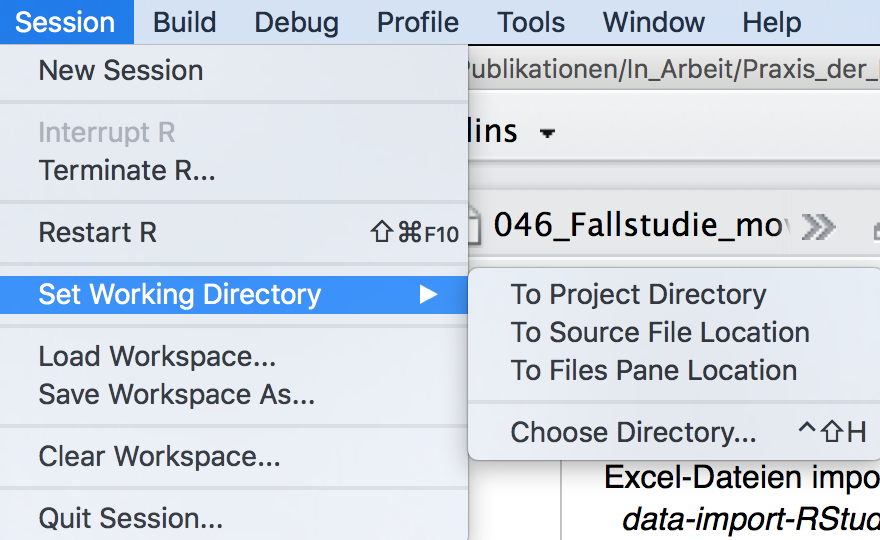
\includegraphics[width=0.5\linewidth]{images/tidy/Arbeitsverzeichnis} 

}

\caption{Das Arbeitsverzeichnis mit RStudio auswählen}\label{fig:Arbeitsverzeichnis}
\end{figure}

Es ist praktisch, das Arbeitsverzeichnis festzulegen, denn dann kann man
z.B. eine Datendatei einlesen, ohne den Pfad eingeben zu müssen:

\begin{Shaded}
\begin{Highlighting}[]
\CommentTok{# nicht ausführen:}
\NormalTok{daten_deutsch <-}\StringTok{ }\KeywordTok{read.csv}\NormalTok{(}\StringTok{"daten_deutsch.csv"}\NormalTok{, }\DataTypeTok{sep =} \StringTok{";"}\NormalTok{, }\DataTypeTok{dec =} \StringTok{"."}\NormalTok{)}
\end{Highlighting}
\end{Shaded}

R geht dann davon aus, dass sich die Datei \texttt{daten\_deutsch.csv}
im Arbeitsverzeichnis befindet.

Für diesen Kurs ist es sinnvoll, das Arbeitsverzeichnis in einen
``Hauptordner'' zu legen (z.B. ``Praxis\_der\_Datenanalyse''), in dem
Daten und sonstiges Material als Unterordner abgelegt sind.

\BeginKnitrBlock{rmdcaution}
Übrigens: Wenn Sie keinen Pfad angeben, so geht R davon aus, dass die
Daten im aktuellen Verzeichnis (dem \emph{working directory}) liegen.
\EndKnitrBlock{rmdcaution}

\section{Hier werden Sie geholfen}\label{hier-werden-sie-geholfen}

\subsection{Wo finde ich Hilfe?}\label{wo-finde-ich-hilfe}

Es ist keine Schande, nicht alle Befehle der ca. 10,000 R-Pakete
auswendig zu wissen. Schlauer ist, zu wissen, wo man Antworten findet.
Hier eine Auswahl:

\begin{itemize}
\item
  Zu diesen Paketen gibt es gute ``Spickzettel'' (cheatsheets): ggplot2,
  RMarkdown, dplyr, tidyr. Klicken Sie dazu in RStudio auf \emph{Help
  \textgreater{} Cheatsheets \textgreater{} \ldots{}} oder gehen Sie auf
  \url{https://www.rstudio.com/resources/cheatsheets/}.
\item
  In RStudio gibt es eine Reihe (viele) von Tastaturkürzeln (Shortcuts),
  die Sie hier finden: \emph{Tools \textgreater{} Keyboard Shortcuts
  Help}.
\item
  Für jeden Befehl aus einem \emph{geladenen} Paket können Sie mit
  \texttt{help()} die Hilfe-Dokumentation anschauen, also z.B.
  \texttt{help("qplot")}.
\item
  Im Internet finden sich zuhauf Tutorials.
\item
  Der Reiter ``Help'' bei RStudio verweist auf die Hilfe-Seite des
  jeweiligen Pakets bzw. Befehls.
\item
  Die bekannteste Seite um Fragen rund um R zu diskutieren ist
  \url{http://stackoverflow.com}.
\end{itemize}

\subsection{Einfache reproduzierbare Beispiele
(ERBies)}\label{einfache-reproduzierbare-beispiele-erbies}

Sagen wir, Sie haben ein Problem. Mit R. Bevor Sie jemanden bitten, Ihr
Problem zu lösen, haben Sie schon \sout{drei} \sout{dreizehn}
\sout{dreißig} Minuten recherchiert, ohne Erfolg. Sie entschließen sich,
bei \href{www.stackoverflow.com}{Stackoverflow} Ihr Problem zu posten.
Außerdem kann sicher eine Mail zu einem Bekannten, einem Dozenten oder
sonstwem, der sich auskennen sollte, nicht schaden. Sie formulieren also
Ihr Problem: ``Hallo, mein R startet nicht, und wenn es startet, dann
macht es nicht, was ich soll, außerdem funktioniert der Befehl `mean'
bei mir nicht. Bitte lös mein Problem!''. Seltsamerweise reagieren die
Empfänger Ihrer Nachricht nicht alle begeistert. Stattdessen verlangt
jemand (dreist) nach einer genauen Beschreibung Ihres Problems, mit dem
Hinweis, dass ``Ferndiagnosen'' schwierig sein. Genauer gesagt möchte
ihr potenzieller Helfer ein `minimal reproducible example' (MRE) oder,
Deutsch, ein \emph{einfaches reproduzierbares
Beispiel}\index{einfaches reproduzierbares Beispiel} (ERBie).

\begin{quote}
Wenn Sie jemanden um R-Hilfe bitten, dann sollten Sie Ihr Problem
prägnant beschreiben.
\end{quote}

Was sollte alles in einem ERBie enthalten sein?

\begin{quote}
Ein ERBie besteht aus vier Teilen: Syntax, Daten, Paketen und Infos zum
laufenden System (R Version etc.)
\end{quote}

Wie sollte so ein ERBie aussehen? Ich empfehle, folgende Eckpunkte zu
beachten\footnote{Hier finden Sie weitere Hinweise zu ERBies:
  \url{https://stackoverflow.com/help/mcve} oder
  \url{https://gist.github.com/hadley/270442}}:

\begin{itemize}
\tightlist
\item
  Syntax: Stellen Sie die R-Syntax bereit, die ein Problem bereit (d.h.
  die einen Fehler liefert).
\item
  Einfach: Geben Sie sowenig Syntax wie möglich an. Es bereitet Ihrem
  Helfer nur wenig Spaß, sich durch 2000 Zeilen Code zu wühlen, wenn es
  10 Zeilen auch getan hätten.
\item
  Reproduzierbar Geben Sie soviel Syntax wie nötig, um den Fehler zu
  erzeugen (aber nicht mehr).
\item
  Schreiben Sie Ihre Syntax übersichtlich, veständlich und kommentiert;
  z.B. sollten die Variablennamen informativ sein.
\item
  Beschreiben Sie den Fehler genau (``läuft nicht'' reicht nicht); z.B.
  ist es hilfreich, den Wortlaut einer Fehlermeldung bereitzustellen.
\item
  Zu Beginn der Syntax sollten die benötigten Pakete geladen werden.
\item
  Zu Ende des ERBie sollte der Output von \texttt{sessionInfo()}
  einkopiert werden; damit werden Informationen zum laufenden System
  (wie Version von R, Betriebssystem etc.) bereitgestellt.
\item
  Beziehen Sie sich möglichst auf Daten, die in R schon ``eingebaut
  sind'' wie die Datensätze \texttt{iris} oder \texttt{mtcars}.
\end{itemize}

Natürlich sollte man immer erst selbst nach einer Lösung recherchieren,
bevor man jemanden um Hilfe bittet. Viele Fragen wurden schon einmal
diskutiert und oft auch gelöst.

\section{Was ist Statistik? Wozu ist sie
gut?}\label{was-ist-statistik-wozu-ist-sie-gut}

Zwei Fragen bieten sich sich am Anfang der Beschäftigung mit jedem Thema
an: Was ist die Essenz des Themas? Warum ist das Thema (oder die
Beschäftigung damit) wichtig?

Was ist Statistik? \emph{Eine} Antwort dazu ist, dass Statistik die
Wissenschaft von Sammlung, Analyse, Interpretation und Kommunikation von
Daten ist mithilfe mathematischer Verfahren ist und zur
Entscheidungshilfe beitragen solle (\emph{The Oxford Dictionary of
Statistical Terms} \protect\hyperlink{ref-oxford}{2006}; Romeijn
\protect\hyperlink{ref-sep-statistics}{2016}). Damit hätten wir auch den
Unterschied zur schnöden Datenanalyse (ein Teil der Statistik)
herausgemeißelt. Statistik wird häufig in die zwei Gebiete
\emph{deskriptive} und \emph{inferierende} Statistik eingeteilt (vgl.
Abb. \ref{fig:desk-vs-inf}). Erstere fasst viele Zahlen zusammen, so
dass wir den Wald statt vieler Bäume sehen. Letztere verallgemeinert von
den vorliegenden (sog. ``Stichproben-'')Daten auf eine zugrunde liegende
Grundmenge (Population). Dabei spielt die Wahrscheinlichkeitsrechnung
(Stochastik) eine große Rolle.

\begin{figure}

{\centering 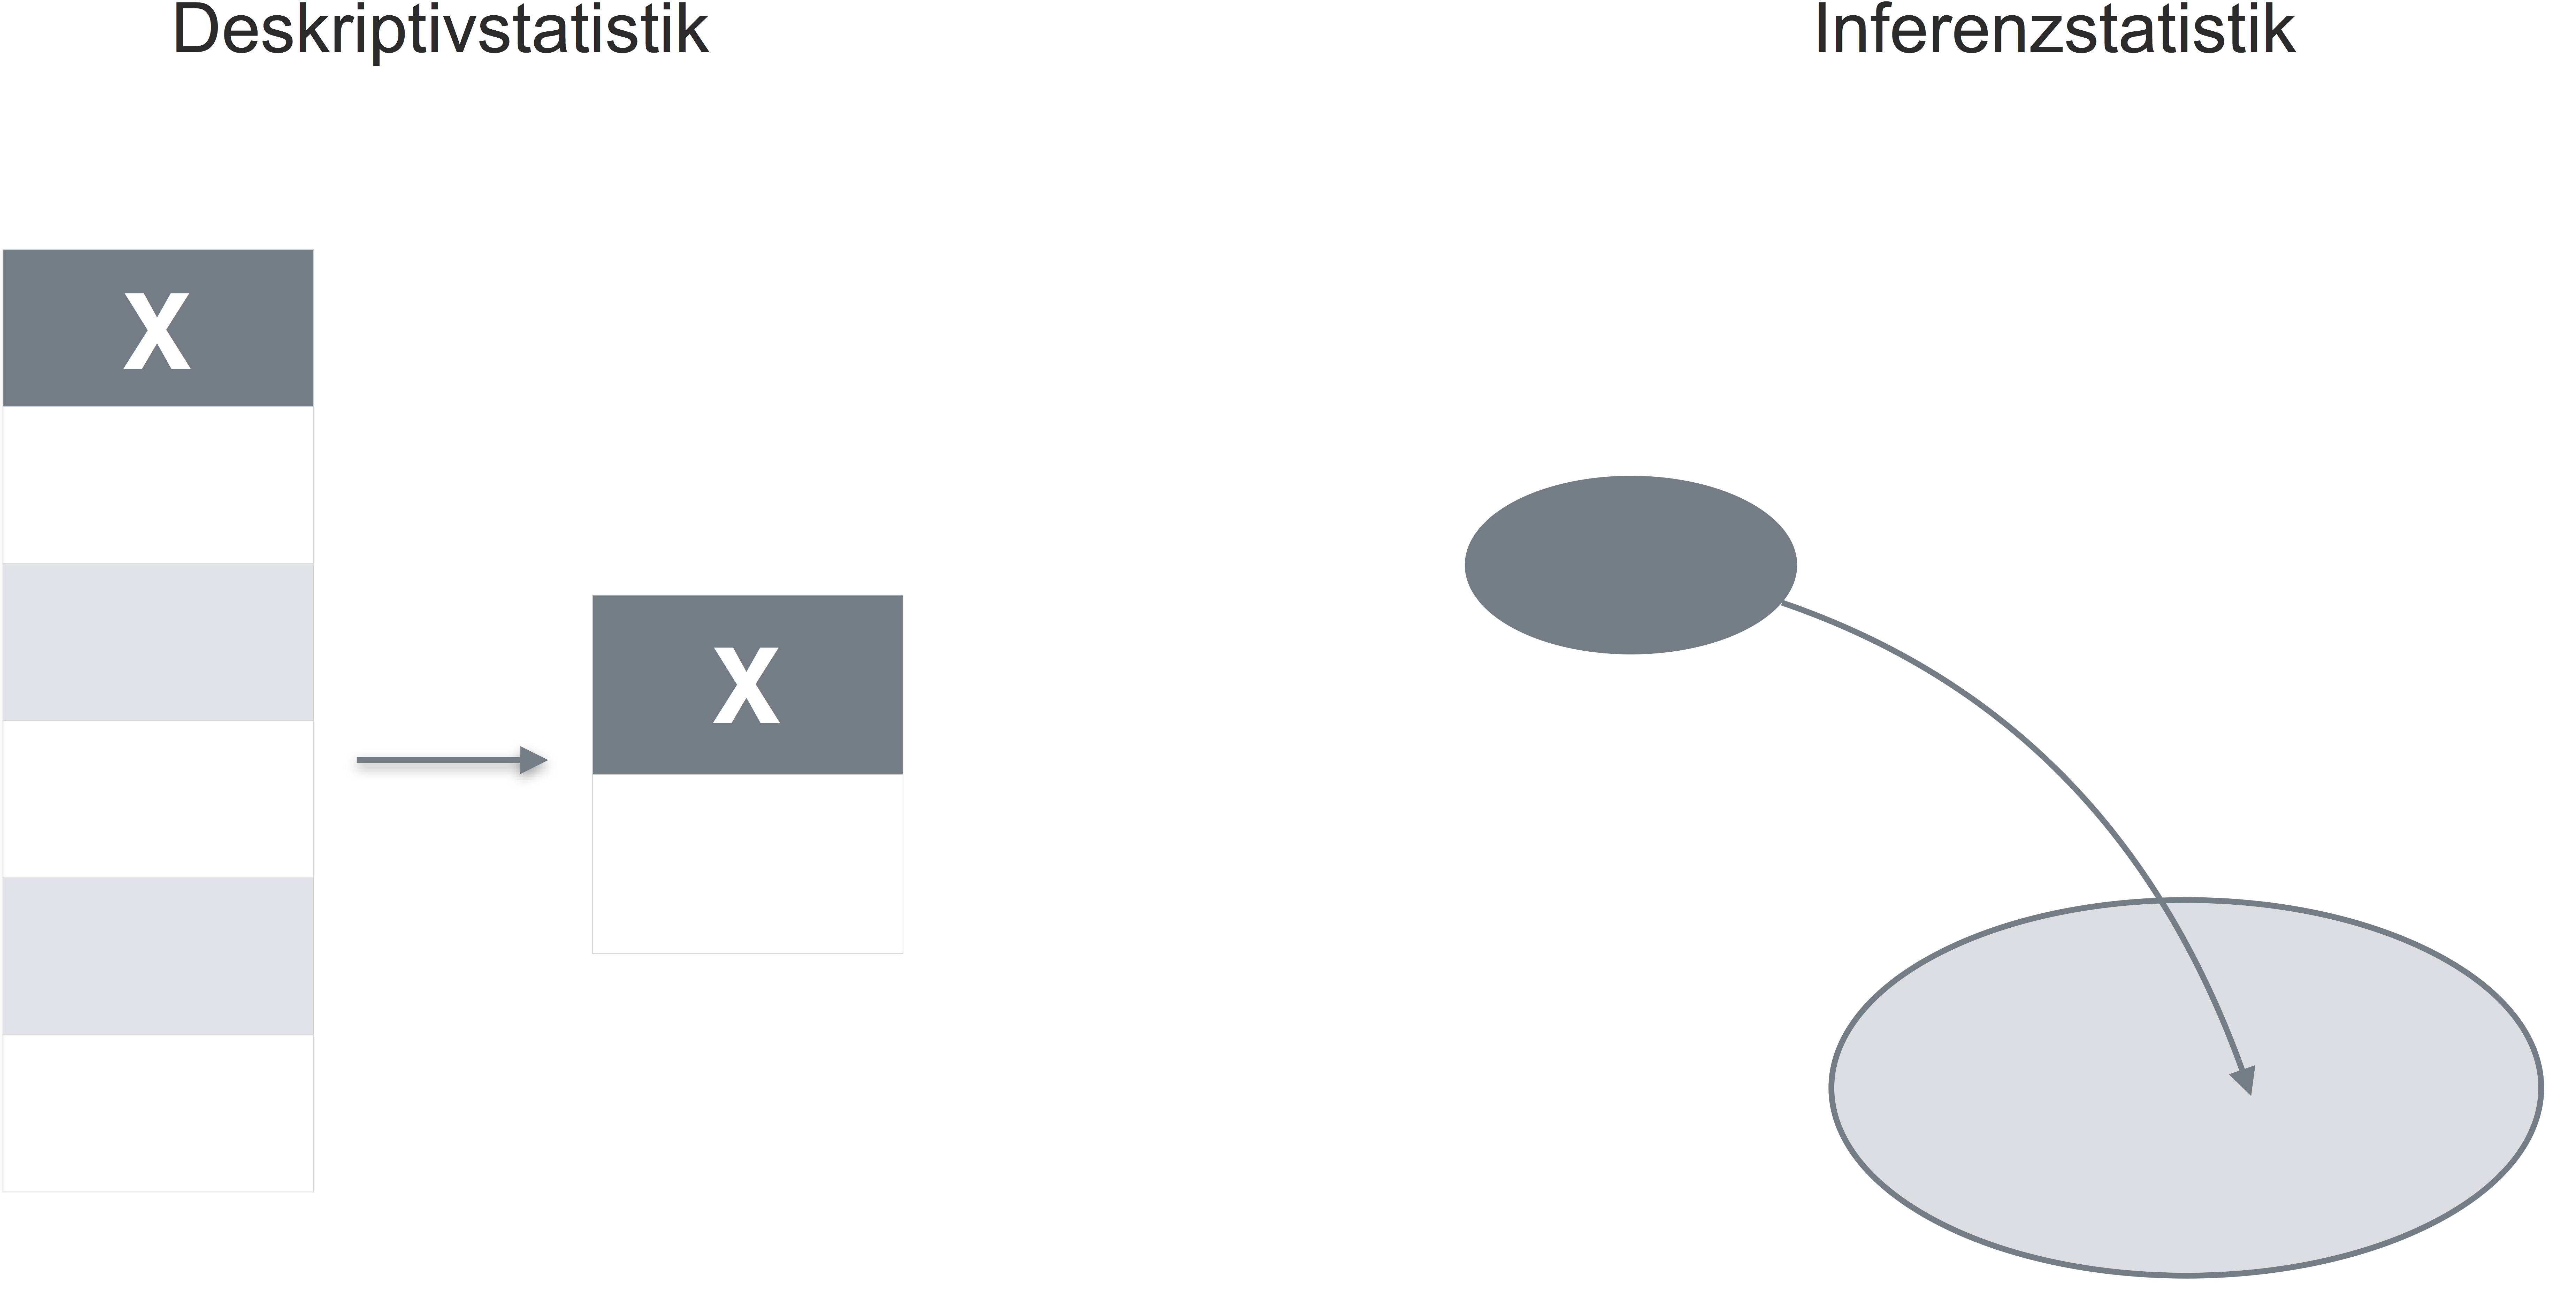
\includegraphics[width=0.7\linewidth]{images/Rahmen/desk_vs_inf-crop} 

}

\caption{Sinnbild für die Deskriptiv- und die Inferenzstatistik}\label{fig:desk-vs-inf}
\end{figure}

Aufgabe der deskriptiven Statistik ist es primär, Daten prägnant
zusammenzufassen. Aufgabe der Inferenzstatistik ist es, zu prüfen, ob
Daten einer Stichprobe auf eine Grundgesamtheit verallgemeinert werden
können.

Dabei lässt sich der Begriff ``Statistik'' als Überbegriff von
``Datenanalyse'' verstehen, wenn diese Sicht auch nicht von allen
geteilt wird (Grolemund und Wickham
\protect\hyperlink{ref-grolemund2014cognitive}{2014}). In diesem Buch
steht die Aufbereitung, Analyse, Interpretation und Kommunikation von
Daten im Vordergrund. Liegt der Schwerpunkt dieser Aktivitäten bei
computerintensiven Methoden, so wird auch von \emph{Data Science}
gesprochen, wobei der Begriff nicht einheitlich verwendet wird (Wickham
und Grolemund \protect\hyperlink{ref-r4ds}{2016}; Hardin u.~a.
\protect\hyperlink{ref-hardin2015data}{2015})

\emph{Daten} kann man definieren als \emph{Informationen, die in einem
Kontext stehen} (Moore
\protect\hyperlink{ref-moore1990uncertainty}{1990}), wobei eine
numerische Konnotation mitschwingt.

\emph{Modellieren} kann man als \emph{zentrale Aufgabe von Statistik}
begreifen (Cobb \protect\hyperlink{ref-cobb2007introductory}{2007};
Grolemund und Wickham
\protect\hyperlink{ref-grolemund2014cognitive}{2014}). Einfach
gesprochen, bedeutet Modellieren in diesem Sinne, ein mathematisches
Narrativ (``Geschichte'') zu finden, welches als Erklärung für gewisse
Muster in den Daten fungiert; vgl. Kap. \ref{mod1}.

Statistisches Modellieren läuft gewöhnlich nach folgendem Muster ab
(Grolemund und Wickham
\protect\hyperlink{ref-grolemund2014cognitive}{2014}):

\begin{verbatim}
Prämisse 1: Wenn Modell M wahr ist, dann sollten die Daten das Muster D aufweisen.
Prämisse 2: Die Daten weisen das Muster D auf.
---
Konklusion: Daher muss das Modell M wahr sein.
\end{verbatim}

Die Konklusion ist \emph{nicht} zwangsläufig richtig. Es ist falsch zu
sagen, dass dieses Argumentationsmuster - Abduktion (Peirce
\protect\hyperlink{ref-peirce1955abduction}{1955}) genannt - wahre,
sichere Schlüsse (Konklusionen) liefert. Die Konklusion \emph{kann, muss
aber nicht}, zutreffen.

Ein Beispiel: Auf dem Nachhauseweg eines langen Arbeitstags wartet, in
einer dunklen Ecke, ein Mann, der sich als Statistik-Professor vorstellt
und Sie zu einem Glücksspiel einlädt. Sofort sagen Sie zu. Der
Statistiker will 10 Mal eine Münze werfen, er setzt auf Zahl (versteht
sich). Wenn er gewinnt, bekommt er 10\euro{} von Ihnen; gewinnen Sie,
bekommen Sie 11\euro{} von ihm. Hört sich gut an, oder? Nun wirft er die
Münze zehn Mal. Was passiert? Er gewinnt 10 Mal, natürlich (so will es
die Geschichte). Sollten wir glauben, dass er ein Betrüger ist?

Ein Modell, welches wir hier verwenden könnten, lautet: Wenn die Münze
gezinkt ist (Modell M zutrifft), dann wäre diese Datenlage D (10 von 10
Treffern) wahrscheinlich - Prämisse 1. Datenlage D ist tatsächlich der
Fall; der Statistiker hat 10 von 10 Treffer erzielt - Prämisse 2. Die
Daten D ``passen'' also zum Modell M; man entscheidet sich, dass der
Professor ein Falschspieler ist.

Wichtig zu erkennen ist, dass Abduktion mit dem Wörtchen \emph{wenn}
beginnt. Also davon \emph{ausgeht}, dass ein Modell M der Fall ist (der
Professor also tatsächlich ein Betrüger ist). Das, worüber wir
entscheiden wollen, wird bereits vorausgesetzt. Falls M gilt, gehen wir
mal davon aus, wie gut passen dann die Daten dazu?

\begin{quote}
Wie gut passen die Daten D zum Modell M?
\end{quote}

Das ist die Frage, die hier tatsächlich gestellt bzw. beantwortet wird.

Natürlich ist es keineswegs sicher, \emph{dass} das Modell gilt. Darüber
macht die Abduktion auch keine Aussage. Es könnte also sein, dass ein
anderes Modell zutrifft: Der Professor könnte ein Heiliger sein, der uns
auf etwas merkwürdige Art versucht, Geld zuzuschanzen\ldots{} Oder er
hat einfach Glück gehabt.

\begin{quote}
Statistische Modelle beantworten i.d.R. nicht, wie wahrscheinlich es
ist, dass ein Modell gilt. Statistische Modelle beurteilen, wie gut
Daten zu einem Modell passen.
\end{quote}

Häufig trifft ein Modell eine Reihe von Annahmen, die nicht immer
explizit gemacht werden, aber die klar sein sollten. Z.B. sind die
Münzwürfe unabhängig voneinander? Oder kann es sein, dass sich die Münze
``einschießt'' auf eine Seite? Dann wären die Münzwürfe nicht unabhängig
voneinander. In diesem Fall klingt das reichlich unplausibel; in anderen
Fällen kann dies eher der Fall sein\footnote{Sind z.B. die
  Prüfungsergebnisse von Schülern unabhängig voneinander? Möglicherweise
  haben sie von einem ``Superschüler'' abgeschrieben. Wenn der
  Superschüler viel weiß, dann zeigen die Abschreiber auch gute
  Leistung.}. Auch wenn die Münzwürfe unabhängig voneinander sind, ist
die Wahrscheinlichkeit für Zahl jedes Mal gleich? Hier ist es wiederum
unwahrscheinlich, dass sich die Münze verändert, ihre Masse verlagert,
so dass eine Seite Unwucht bekommt. In anderen Situationen können sich
Untersuchungsobjekte verändern (Menschen lernen manchmal etwas, sagt
man), so dass die Wahrscheinlichkeiten für ein Ereignis unterschiedlich
sein können, man dies aber nicht berücksichtigt.

\section{Aufgaben}\label{aufgaben}

\begin{enumerate}
\def\labelenumi{\arabic{enumi}.}
\item
  Öffnen Sie das Cheatsheet für RStudio und machen Sie sich mit dem
  Cheatsheet vertraut.
\item
  Sichten Sie kurz die übrigen Cheatsheets; später werden die Ihnen
  vielleicht von Nutzen sein.
\item
  Führen Sie diese Syntax aus:
\end{enumerate}

\begin{Shaded}
\begin{Highlighting}[]
\NormalTok{meine_coole_variable <-}\StringTok{ }\DecValTok{10}
\NormalTok{meine_coole_var1able }
\end{Highlighting}
\end{Shaded}

Woher rührt der Fehler?

\begin{enumerate}
\def\labelenumi{\arabic{enumi}.}
\setcounter{enumi}{3}
\tightlist
\item
  Korrigieren Sie die Syntax:
\end{enumerate}

\begin{Shaded}
\begin{Highlighting}[]
\KeywordTok{install.packages}\NormalTok{(dplyer)}
\end{Highlighting}
\end{Shaded}

\texttt{y\ \textless{}-\ Hallo\ R!}

\texttt{Hallo\ R\ \textless{}-\ 1}

\begin{Shaded}
\begin{Highlighting}[]
\NormalTok{Hallo_R }\OperatorTok{<}\StringTok{ }\OperatorTok{-}\StringTok{ }\DecValTok{1}
\end{Highlighting}
\end{Shaded}

Richtig oder Falsch???\footnote{R, F: die Daten müssen sinnvoll
  zusammengefasst werden, F, F, F: Wenn er ehrlich sein sollte, dann ist
  das Ereignis `10 von 10' selten}

\BeginKnitrBlock{rmdexercises}
Richtig oder Falsch!?

\begin{enumerate}
\def\labelenumi{\arabic{enumi}.}
\item
  Statistik wird gemeinhin in zwei Bereiche unterteilt:
  Deskriptivstatistik und Inferenzstatistik.
\item
  Unter Deskriptivstatistik versteht man, Daten zu beschreiben. Dazu ist
  jede Art von Beschreibung sinnvoll, vorausgesetzt es wird eine
  konsistente Regel eingesetzt.
\item
  Unter Abduktion versteht man den Schluss vom Allgemeinen auf das
  Konkrete.
\item
  Wirft jemand bei 10 von 10 Münzwürfen `Kopf', so muss er ein Betrüger
  sein.
\item
  Wirft jemand bei 10 von 10 Münzwürfen `Kopf', so ist die
  Wahrscheinlichkeit groß, dass er ein Betrüger ist.
\end{enumerate}
\EndKnitrBlock{rmdexercises}

\section{Befehlsübersicht}\label{befehlsubersicht}

Tabelle \ref{tab:befehle-rahmen} stellt die Befehle dieses Kapitels dar.

\begin{table}

\caption{\label{tab:befehle-rahmen}Befehle des Kapitels 'Rahmen'}
\centering
\begin{tabular}[t]{l|l}
\hline
Paket::Funktion & Beschreibung\\
\hline
install.packages("x") & Installiert Paket "x" (nicht: Paket "X")\\
\hline
library & lädt ein Paket\\
\hline
<- & Weist einer Variablen einen Wert zu\\
\hline
c & erstellt eine Spalte/ einen Vektor\\
\hline
\end{tabular}
\end{table}

Diese Befehle ``wohnen'' alle im Standard-R; es ist für diese Befehle
nicht nötig, zusätzliche Pakete zu installieren/ laden.

\section{Verweise}\label{verweise}

\begin{itemize}
\item
  Chester Ismay erläutert einige Grundlagen von R und RStudio, die für
  Datenanalyse hilfreich sind:
  \url{https://bookdown.org/chesterismay/rbasics/}.
\item
  Roger Peng und Kollegen bieten hier einen Einstieg in Data Science mit
  R: \url{https://bookdown.org/rdpeng/artofdatascience/}
\item
  Wickham und Grolemund (\protect\hyperlink{ref-r4ds}{2016}) geben einen
  hervorragenden Überblick in das Thema dieses Buches; ihr Buch ist sehr
  zu empfehlen.
\item
  Wer einen stärker an der Statistik orientierten Zugang sucht, aber
  ``mathematisch sanft'' behandelt werden möchte, wird bei James et al.
  (\protect\hyperlink{ref-introstatlearning}{2013}\protect\hyperlink{ref-introstatlearning}{b})
  glücklich oder zumindest fündig werden.
\item
  Uwe Ligges (\emph{Programmieren mit R}
  \protect\hyperlink{ref-ligges}{2009}) `Programmieren mit R' gibt einen
  tieferen Einstieg in die Grundlagen von R.
\item
  Wer ganz tief ein- und abtauchen möchte in R, dem sei - solide
  Grundkenntnisse vorausgesetzt - Hadley Wickhams Wickham
  (\protect\hyperlink{ref-wickham2014advanced}{2014}\protect\hyperlink{ref-wickham2014advanced}{a})
  `Advanced R' ans Herz gelegt.
\end{itemize}

\chapter{Daten einlesen}\label{daten-einlesen}

\chapter{Datenjudo}\label{Datenjudo}

\chapter{Praxisprobleme der
Datenaufbereitung}\label{praxisprobleme-der-datenaufbereitung}

\chapter{\texorpdfstring{Fallstudie
`movies'}{Fallstudie movies}}\label{case-movies}

\chapter{Daten visualisieren}\label{daten-visualisieren}

\chapter{Fallstudie zur
Visualisierung}\label{fallstudie-zur-visualisierung}

\chapter{Grundlagen des Modellierens}\label{mod1}

\chapter{Der p-Wert, Inferenzstatistik und
Alternativen}\label{der-p-wert-inferenzstatistik-und-alternativen}

\chapter{Lineare Regression}\label{lineare-regression}

\chapter{Klassifizierende Regression}\label{klassifizierende-regression}

\chapter{Fallstudien zum geleiteten
Modellieren}\label{fallstudien-zum-geleiteten-modellieren}

\chapter{Vertiefung: Clusteranalyse}\label{cluster}

\chapter{Vertiefung:
Dimensionsreduktion}\label{vertiefung-dimensionsreduktion}

\chapter{Vertiefung: Grundlagen des
Textmining}\label{vertiefung-grundlagen-des-textmining}

\chapter{Placeholder}\label{placeholder-1}

\chapter{Probeklausur}\label{probeklausur}

\chapter{Hinweise}\label{hinweise-1}

\chapter{Literaturverzeichnis}\label{literaturverzeichnis}

\hypertarget{refs}{}
\hypertarget{ref-R-rmarkdown}{}
Allaire, JJ, Joe Cheng, Yihui Xie, Jonathan McPherson, Winston Chang,
Jeff Allen, Hadley Wickham, Aron Atkins, und Rob Hyndman. 2016a.
\emph{rmarkdown: Dynamic Documents for R}.
\url{https://CRAN.R-project.org/package=rmarkdown}.

\hypertarget{ref-rmarkdown}{}
---------. 2016b. \emph{rmarkdown: Dynamic Documents for R}.
\url{https://CRAN.R-project.org/package=rmarkdown}.

\hypertarget{ref-R-gridExtra}{}
Auguie, Baptiste. 2016. \emph{gridExtra: Miscellaneous Functions for
„Grid`` Graphics}. \url{https://CRAN.R-project.org/package=gridExtra}.

\hypertarget{ref-R-BaylorEdPsych}{}
Beaujean, A. Alexander. 2012. \emph{BaylorEdPsych: R Package for Baylor
University Educational Psychology Quantitative Courses}.
\url{https://CRAN.R-project.org/package=BaylorEdPsych}.

\hypertarget{ref-R-quanteda}{}
Benoit, Kenneth, und Paul Nulty. 2016. \emph{quanteda: Quantitative
Analysis of Textual Data}.
\url{https://CRAN.R-project.org/package=quanteda}.

\hypertarget{ref-R-SnowballC}{}
Bouchet-Valat, Milan. 2014. \emph{SnowballC: Snowball stemmers based on
the C libstemmer UTF-8 library}.
\url{https://CRAN.R-project.org/package=SnowballC}.

\hypertarget{ref-breaking}{}
Briggs, William M. 2008a. \emph{Breaking the Law of Averages: Real-Life
Probability and Statistics in Plain English}. Lulu.com.

\hypertarget{ref-Breaking}{}
---------. 2008b. \emph{Breaking the Law of Averages: Real-Life
Probability and Statistics in Plain English}. Lulu.com.
\url{https://www.amazon.com/Breaking-Law-Averages-Probability-Statistics/dp/0557019907?SubscriptionId=0JYN1NVW651KCA56C102\&tag=techkie-20\&linkCode=xm2\&camp=2025\&creative=165953\&creativeASIN=0557019907}.

\hypertarget{ref-uncertainty}{}
---------. 2016. \emph{Uncertainty: The Soul of Modeling, Probability \&
Statistics}. Springer.

\hypertarget{ref-bryant1995practical}{}
Bryant, PG, und MA Smith. 1995. „Practical Data Analysis: Case Studies
in Business Statistics, Homewood, IL: Richard D``. Irwin Publishing.

\hypertarget{ref-R-downloader}{}
Chang, Winston. 2015. \emph{downloader: Download Files over HTTP and
HTTPS}. \url{https://CRAN.R-project.org/package=downloader}.

\hypertarget{ref-Chapman2015}{}
Chapman, Chris, und Elea McDonnell Feit. 2015. \emph{R for Marketing
Research and Analytics}. New York City: Springer.
doi:\href{https://doi.org/10.1007/978-3-319-14436-8}{10.1007/978-3-319-14436-8}.

\hypertarget{ref-Cleveland}{}
Cleveland, William S. 1993. \emph{Visualizing Data}. Hobart Press.

\hypertarget{ref-clopper1934use}{}
Clopper, Charles J, und Egon S Pearson. 1934. „The use of confidence or
fiducial limits illustrated in the case of the binomial``.
\emph{Biometrika} 26 (4). JSTOR: 404--13.

\hypertarget{ref-cobb2007introductory}{}
Cobb, George W. 2007. „The introductory statistics course: a Ptolemaic
curriculum?`` \emph{Technology Innovations in Statistics Education} 1
(1).

\hypertarget{ref-Cohen1992}{}
Cohen, J. 1992. „A power primer``. \emph{Psychological Bulletin} 112
(1): 155--59.

\hypertarget{ref-cohen_statistical_1988}{}
Cohen, Jacob. 1988. \emph{Statistical Power Analysis for the Behavioral
Sciences}. Routledge. \url{http://dx.doi.org/10.4324/9780203771587}.

\hypertarget{ref-cortez2009modeling}{}
Cortez, Paulo, António Cerdeira, Fernando Almeida, Telmo Matos, und José
Reis. 2009. „Modeling wine preferences by data mining from
physicochemical properties``. \emph{Decision Support Systems} 47 (4).
Elsevier: 547--53.

\hypertarget{ref-R-ggdendro}{}
de Vries, Andrie, und Brian D. Ripley. 2016. \emph{ggdendro: Create
Dendrograms and Tree Diagrams Using 'ggplot2'}.
\url{https://CRAN.R-project.org/package=ggdendro}.

\hypertarget{ref-introstats}{}
Diez, David M, Christopher D Barr, und Mine Cetinkaya-Rundel. 2014.
\emph{Introductory Statistics with Randomization and Simulation}. North
Charleston, South Carolina: CreateSpace Independent Publishing Platform.

\hypertarget{ref-eid2010statistik}{}
Eid, Michael, Mario Gollwitzer, und Manfred Schmitt. 2010.
\emph{Statistik und Forschungsmethoden}. Göttingen: Hogrefe.

\hypertarget{ref-etz2016become}{}
Etz, Alexander, Quentin Frederik Gronau, Fabian Dablander, Peter
Edelsbrunner, und Beth Baribault. 2016. „How to become a Bayesian in
eight easy steps: An annotated reading list``. PsyArXiv.

\hypertarget{ref-fair1978theory}{}
Fair, Ray C. 1978. „A theory of extramarital affairs``. \emph{Journal of
Political Economy} 86 (1). The University of Chicago Press: 45--61.

\hypertarget{ref-R-tm}{}
Feinerer, Ingo, und Kurt Hornik. 2015. \emph{tm: Text Mining Package}.
\url{https://CRAN.R-project.org/package=tm}.

\hypertarget{ref-R-wordcloud}{}
Fellows, Ian. 2014. \emph{wordcloud: Word Clouds}.
\url{https://CRAN.R-project.org/package=wordcloud}.

\hypertarget{ref-fjalnes_orthogonale_2014}{}
Fjalnes. 2014. „Orthogonale Faktorrotation``.
\url{https://de.wikipedia.org/wiki/Rotationsverfahren_(Statistik)\#/media/File:Orthogonale_faktorrotation.svg}.

\hypertarget{ref-R-car}{}
Fox, John, und Sanford Weisberg. 2016. \emph{car: Companion to Applied
Regression}. \url{https://CRAN.R-project.org/package=car}.

\hypertarget{ref-Gansser_2017}{}
Gansser, Oliver. 2017. „Data for Principal Component Analysis and Common
Factor Analysis``. Open Science Framework. \url{osf.io/zg89r}.

\hypertarget{ref-gigerenzer1980}{}
Gigerenzer, Gerd. 1980. \emph{Messung und Modellbildung in der
Psychologie (Uni-Taschenbucher. Psychologie, Padagogik, Soziologie,
Psychiatrie) (German Edition)}. E. Reinhardt.

\hypertarget{ref-Gigerenzer2004}{}
---------. 2004. „Mindless statistics``. \emph{The Journal of
Socio-Economics} 33 (5). Elsevier BV: 587--606.
doi:\href{https://doi.org/10.1016/j.socec.2004.09.033}{10.1016/j.socec.2004.09.033}.

\hypertarget{ref-god_i_2016}{}
God. 2016. „I don't care about you. Please share this with friends.``
Twitter Tweet. \emph{TheTweetOfGod}.
\url{https://twitter.com/TheTweetOfGod/status/688035049187454976}.

\hypertarget{ref-grolemund2014cognitive}{}
Grolemund, Garrett, und Hadley Wickham. 2014. „A cognitive
interpretation of data analysis``. \emph{International Statistical
Review} 82 (2). Wiley Online Library: 184--204.

\hypertarget{ref-R-arules}{}
Hahsler, Michael, Christian Buchta, Bettina Gruen, und Kurt Hornik.
2016. \emph{arules: Mining Association Rules and Frequent Itemsets}.
\url{https://CRAN.R-project.org/package=arules}.

\hypertarget{ref-R-arulesViz}{}
Hahsler, Michael, und Sudheer Chelluboina. 2016. \emph{arulesViz:
Visualizing Association Rules and Frequent Itemsets}.
\url{https://CRAN.R-project.org/package=arulesViz}.

\hypertarget{ref-hamermesh2005beauty}{}
Hamermesh, Daniel S, und Amy Parker. 2005. „Beauty in the classroom:
Instructors' pulchritude and putative pedagogical productivity``.
\emph{Economics of Education Review} 24 (4). Elsevier: 369--76.

\hypertarget{ref-hardin2015data}{}
Hardin, Johanna, Roger Hoerl, Nicholas J Horton, Deborah Nolan, Ben
Baumer, Olaf Hall-Holt, Paul Murrell, u.~a. 2015. „Data science in
statistics curricula: Preparing students to 'Think with Data'``.
\emph{The American Statistician} 69 (4). Taylor \& Francis: 343--53.

\hypertarget{ref-Hatzinger}{}
Hatzinger, Reinhold, Kurt Hornik, und Herbert Nagel. 2014. \emph{R-
Einfuehrung durch angewandte Statistik}. Pearson Studium.

\hypertarget{ref-Head2015}{}
Head, Megan L., Luke Holman, Rob Lanfear, Andrew T. Kahn, und Michael D.
Jennions. 2015. „The Extent and Consequences of P-Hacking in Science``.
\emph{PLOS Biology} 13 (3). Public Library of Science (PLoS): e1002106.
doi:\href{https://doi.org/10.1371/journal.pbio.1002106}{10.1371/journal.pbio.1002106}.

\hypertarget{ref-R-titanic}{}
Hendricks, Paul. 2015. \emph{titanic: Titanic Passenger Survival Data
Set}. \url{https://CRAN.R-project.org/package=titanic}.

\hypertarget{ref-hoekstra2014robust}{}
Hoekstra, Rink, Richard D Morey, Jeffrey N Rouder, und Eric-Jan
Wagenmakers. 2014. „Robust misinterpretation of confidence intervals``.
\emph{Psychonomic bulletin \& review} 21 (5). Springer: 1157--64.

\hypertarget{ref-hyndman2014forecasting}{}
Hyndman, R.J., und G. Athanasopoulos. 2014. \emph{Forecasting:
principles and practice:} OTexts.
\url{https://books.google.de/books?id=gDuRBAAAQBAJ}.

\hypertarget{ref-edu_icons}{}
Icon-Pond. 2016. „Education. 35 Icons.`` Flaticon.
\url{http://www.flaticon.com/authors/popcorns-arts}.

\hypertarget{ref-tm}{}
Ingo Feinerer, Kurt Hornik, und David Meyer. 2008. „Text Mining
Infrastructure in R``. \emph{Journal of Statistical Software} 25 (5):
1--54. \url{http://www.jstatsoft.org/v25/i05/}.

\hypertarget{ref-R-corrr}{}
Jackson, Simon. 2016. \emph{corrr: Correlations in R}.
\url{https://CRAN.R-project.org/package=corrr}.

\hypertarget{ref-R-ISLR}{}
James, Gareth, Daniela Witten, Trevor Hastie, und Rob Tibshirani. 2013a.
\emph{ISLR: Data for An Introduction to Statistical Learning with
Applications in R}. \url{https://CRAN.R-project.org/package=ISLR}.

\hypertarget{ref-introstatlearning}{}
James, Gareth, Daniela Witten, Trevor Hastie, und Robert Tibshirani.
2013b. \emph{An introduction to statistical learning}. Bd. 6. Springer.

\hypertarget{ref-james2013introduction}{}
---------. 2013c. \emph{An introduction to statistical learning}. Bd. 6.
Springer.

\hypertarget{ref-tidytextminig}{}
Julia, PhD Silge, und PhD Robinson David. 2017. \emph{Text Mining with
R: A tidy approach}. O'Reilly Media.

\hypertarget{ref-Kerby2014}{}
Kerby, Dave S. 2014. „The Simple Difference Formula: An Approach to
Teaching Nonparametric Correlation``. \emph{Comprehensive Psychology} 3:
11.IT.3.1.
doi:\href{https://doi.org/10.2466/11.IT.3.1}{10.2466/11.IT.3.1}.

\hypertarget{ref-kim2015okcupid}{}
Kim, Albert Y, und Adriana Escobedo-Land. 2015. „OkCupid Data for
Introductory Statistics and Data Science Courses``. \emph{Journal of
Statistics Education} 23 (2). Citeseer: n2.

\hypertarget{ref-R-okcupiddata}{}
Kim, Albert Y., und Adriana Escobedo-Land. 2016. \emph{okcupiddata:
OkCupid Profile Data for Introductory Statistics and Data Science
Courses}. \url{https://CRAN.R-project.org/package=okcupiddata}.

\hypertarget{ref-kraemer2011wir}{}
Krämer, W. 2011. \emph{Wie wir uns von falschen Theorien täuschen
lassen}. Berlin University Press.
\url{https://books.google.de/books?id=HWUKaAEACAAJ}.

\hypertarget{ref-kruschke2010bayesian}{}
Kruschke, John K. 2010. „Bayesian data analysis``. \emph{Wiley
Interdisciplinary Reviews: Cognitive Science} 1 (5). Burlington, MA:
Academic Press: 658--76.

\hypertarget{ref-kuhn2013applied}{}
Kuhn, Max, und Kjell Johnson. 2013. \emph{Applied predictive modeling}.
Bd. 26. Springer.

\hypertarget{ref-R-scatterplot3d}{}
Ligges, Uwe, Martin Maechler, und Sarah Schnackenberg. 2017.
\emph{scatterplot3d: 3D Scatter Plot}.
\url{https://CRAN.R-project.org/package=scatterplot3d}.

\hypertarget{ref-lubke2014angewandte}{}
Lübke, Karsten, und Martin Vogt. 2014. \emph{Angewandte
Wirtschaftsstatistik: Daten und Zufall}. Berlin: Springer.

\hypertarget{ref-m7_savinellis_2004}{}
M7. 2004. „Savinelli's Italian smoking pipe``.
\url{https://commons.wikimedia.org/wiki/File:Pipa_savinelli.jpg}.

\hypertarget{ref-matejka2017same}{}
Matejka, Justin, und George Fitzmaurice. 2017. „Same stats, different
graphs: Generating datasets with varied appearance and identical
statistics through simulated annealing``. In \emph{Proceedings of the
2017 CHI Conference on Human Factors in Computing Systems}, 1290--4.
ACM.

\hypertarget{ref-Micceri1989}{}
Micceri, Theodore. 1989. „The unicorn, the normal curve, and other
improbable creatures.`` \emph{Psychological Bulletin} 105 (1): 156--66.
doi:\href{https://doi.org/10.1037/0033-2909.105.1.156}{10.1037/0033-2909.105.1.156}.

\hypertarget{ref-Michell2000}{}
Michell, Joel. 2000. „Normal Science, Pathological Science and
Psychometrics``. \emph{Theory \& Psychology} 10 (5): 639--67.

\hypertarget{ref-R-rpart.plot}{}
Milborrow, Stephen. 2017. \emph{rpart.plot: Plot 'rpart' Models: An
Enhanced Version of 'plot.rpart'}.
\url{https://CRAN.R-project.org/package=rpart.plot}.

\hypertarget{ref-moore1990uncertainty}{}
Moore, David S. 1990. „Uncertainty``. \emph{On the shoulders of giants:
New approaches to numeracy}. ERIC, 95--137.

\hypertarget{ref-R-tokenizers}{}
Mullen, Lincoln. 2016. \emph{tokenizers: A Consistent Interface to
Tokenize Natural Language Text}.
\url{https://CRAN.R-project.org/package=tokenizers}.

\hypertarget{ref-R-RColorBrewer}{}
Neuwirth, Erich. 2014. \emph{RColorBrewer: ColorBrewer Palettes}.
\url{https://CRAN.R-project.org/package=RColorBrewer}.

\hypertarget{ref-Neyman1933}{}
Neyman, J., und E. S. Pearson. 1933. „On the Problem of the Most
Efficient Tests of Statistical Hypotheses``. \emph{Philosophical
Transactions of the Royal Society A: Mathematical, Physical and
Engineering Sciences} 231 (694-706): 289--337.
doi:\href{https://doi.org/10.1098/rsta.1933.0009}{10.1098/rsta.1933.0009}.

\hypertarget{ref-neyman1935problem}{}
Neyman, Jerzy. 1935. „On the problem of confidence intervals``.
\emph{The annals of mathematical statistics} 6 (3). JSTOR: 111--16.

\hypertarget{ref-neyman1992problem}{}
Neyman, Jerzy, und Egon S Pearson. 1992. „On the problem of the most
efficient tests of statistical hypotheses``. In \emph{Breakthroughs in
statistics}, 73--108. New York City: Springer.

\hypertarget{ref-R-pdftools}{}
Ooms, Jeroen. 2016. \emph{pdftools: Text Extraction and Rendering of PDF
Documents}. \url{https://CRAN.R-project.org/package=pdftools}.

\hypertarget{ref-peirce1955abduction}{}
Peirce, Charles S. 1955. „Abduction and induction``. \emph{Philosophical
writings of Peirce} 11. New York.

\hypertarget{ref-peng2015art}{}
Peng, Roger D, und Elizabeth Matsui. 2015. „The Art of Data Science``.
\emph{A Guide for Anyone Who Works with Data. Skybrude Consulting} 200:
162.

\hypertarget{ref-welchertest}{}
Prel, Jean-Baptist du, Bernd Roehrig, Gerhard Hommel, und Maria
Blettner. 2010. \emph{Deutsches Aerzteblatt Online}, Mai. Deutscher
Aerzte-Verlag.
doi:\href{https://doi.org/10.3238/arztebl.2010.0343}{10.3238/arztebl.2010.0343}.

\hypertarget{ref-ligges}{}
\emph{Programmieren mit R}. 2009. Springer Berlin Heidelberg.
doi:\href{https://doi.org/10.1007/978-3-540-79998-6}{10.1007/978-3-540-79998-6}.

\hypertarget{ref-R-nFactors}{}
Raiche, Gilles, und David Magis. 2011. \emph{nFactors: Parallel Analysis
and Non Graphical Solutions to the Cattell Scree Test}.
\url{https://CRAN.R-project.org/package=nFactors}.

\hypertarget{ref-R-wesanderson}{}
Ram, Karthik, und Hadley Wickham. 2015. \emph{wesanderson: A Wes
Anderson Palette Generator}.
\url{https://CRAN.R-project.org/package=wesanderson}.

\hypertarget{ref-R-compute.es}{}
Re, AC Del. 2014. \emph{compute.es: Compute Effect Sizes}.
\url{https://CRAN.R-project.org/package=compute.es}.

\hypertarget{ref-remquahey2010}{}
Remus, R., U. Quasthoff, und G. Heyer. 2010. „SentiWS -- a Publicly
Available German-language Resource for Sentiment Analysis``. In
\emph{Proceedings of the 7th International Language Resources and
Evaluation (LREC'10)}, 1168--71.

\hypertarget{ref-R-MASS}{}
Ripley, Brian. 2016. \emph{MASS: Support Functions and Datasets for
Venables and Ripley's MASS}.
\url{https://CRAN.R-project.org/package=MASS}.

\hypertarget{ref-nycflights13}{}
RITA, Bureau of transportation statistics. 2013. „nycflights13``.
\url{http://www.transtats.bts.gov/DL_SelectFields.asp?Table_ID=236}.

\hypertarget{ref-R-gutenbergr}{}
Robinson, David. 2016. \emph{gutenbergr: Download and Process Public
Domain Works from Project Gutenberg}.
\url{https://cran.rstudio.com/package=gutenbergr}.

\hypertarget{ref-R-broom}{}
Robinson, David, Matthieu Gomez, Boris Demeshev, Dieter Menne, Benjamin
Nutter, Luke Johnston, Ben Bolker, Francois Briatte, und Hadley Wickham.
2015. \emph{broom: Convert Statistical Analysis Objects into Tidy Data
Frames}. \url{https://CRAN.R-project.org/package=broom}.

\hypertarget{ref-R-tidytext}{}
Robinson, David, und Julia Silge. 2016. \emph{tidytext: Text Mining
using 'dplyr', 'ggplot2', and Other Tidy Tools}.
\url{https://CRAN.R-project.org/package=tidytext}.

\hypertarget{ref-sep-statistics}{}
Romeijn, Jan-Willem. 2016. „Philosophy of Statistics``. In \emph{The
Stanford Encyclopedia of Philosophy}, herausgegeben von Edward N. Zalta,
Winter 2016.
\url{http://plato.stanford.edu/archives/win2016/entries/statistics/}.

\hypertarget{ref-ruckerinfinity}{}
Rucker, Rudy. 2004. \emph{Infinity and the Mind}. Princeton: Princeton
University Press. \url{https://books.google.de/books?id=MD0UAwAAQBAJ}.

\hypertarget{ref-Sauer_2016}{}
Sauer, Sebastian. 2016. „Extraversion Dataset``. Open Science Framework.
doi:\href{https://doi.org/10.17605/OSF.IO/4KGZH}{10.17605/OSF.IO/4KGZH}.

\hypertarget{ref-Sauer_2017}{}
---------. 2017a. „Dataset 'predictors of performance in stats test'``.
Open Science Framework.
doi:\href{https://doi.org/10.17605/OSF.IO/SJHUY}{10.17605/OSF.IO/SJHUY}.

\hypertarget{ref-Sauer_2017a}{}
---------. 2017b. „Dataset 'Height and shoe size'``. Open Science
Framework.
doi:\href{https://doi.org/10.17605/OSF.IO/JA9DW}{10.17605/OSF.IO/JA9DW}.

\hypertarget{ref-sauer_wolff}{}
Sauer, Sebastian, und Alexander Wolff. 2016. „The effect of a status
symbol on success in online dating: an experimental study (data
paper)``. \emph{The Winnower}, August.
doi:\href{https://doi.org/10.15200/winn.147241.13309}{10.15200/winn.147241.13309}.

\hypertarget{ref-sauer2010gray}{}
Sauer, Sebastian, Harald Walach, und Niko Kohls. 2010. „Gray's
Behavioural Inhibition System as a mediator of mindfulness towards
well-being``. \emph{Personality and Individual Differences} 50 (4).
Pergamon: 506--51.
doi:\href{https://doi.org/10.1016/j.paid.2010.11.019}{10.1016/j.paid.2010.11.019}.

\hypertarget{ref-R-GGally}{}
Schloerke, Barret, Jason Crowley, Di Cook, Francois Briatte, Moritz
Marbach, Edwin Thoen, Amos Elberg, und Joseph Larmarange. 2016.
\emph{GGally: Extension to 'ggplot2'}.
\url{https://CRAN.R-project.org/package=GGally}.

\hypertarget{ref-Schmidt2007}{}
Schmidt, Peter, Sebastian Bamberg, Eldad Davidov, Johannes Herrmann, und
Shalom H. Schwartz. 2007. „Die Messung von Werten mit dem Portraits
Value Questionnaire``. \emph{Zeitschrift für Sozialpsychologie} 38 (4).
Hogrefe Publishing Group: 261--75.
doi:\href{https://doi.org/10.1024/0044-3514.38.4.261}{10.1024/0044-3514.38.4.261}.

\hypertarget{ref-Shmueli2010}{}
Shmueli, Galit. 2010. „To Explain or to Predict?`` \emph{Statistical
Science} 25 (3): 289--310.
doi:\href{https://doi.org/10.1214/10-STS330}{10.1214/10-STS330}.

\hypertarget{ref-R-janeaustenr}{}
Silge, Julia. 2016. \emph{janeaustenr: Jane Austen's Complete Novels}.
\url{https://CRAN.R-project.org/package=janeaustenr}.

\hypertarget{ref-tidytext-archive}{}
Silge, Julia, David Robinson, und Jim Hester. 2016. „tidytext: Text
mining using dplyr, ggplot2, and other tidy tools``.
doi:\href{https://doi.org/10.5281/zenodo.56714}{10.5281/zenodo.56714}.

\hypertarget{ref-Silge2016}{}
Silge, Julia, und David Robinson. 2016. „tidytext: Text Mining and
Analysis Using Tidy Data Principles in R``. \emph{The Journal of Open
Source Software} 1 (3). The Open Journal.
doi:\href{https://doi.org/10.21105/joss.00037}{10.21105/joss.00037}.

\hypertarget{ref-spurzem_vw_2017}{}
Spurzem, Lothar. 2017. „VW 1303 von Wiking in 1:87``.
\url{https://de.wikipedia.org/wiki/Modellautomobil\#/media/File:Wiking-Modell_VW_1303_(um_1975).JPG}.

\hypertarget{ref-suppes1962basic}{}
Suppes, Patrick, und Joseph L Zinnes. 1962. \emph{Basic measurement
theory}. Institute for mathematical studies in the social sciences.

\hypertarget{ref-oxford}{}
\emph{The Oxford Dictionary of Statistical Terms}. 2006. Oxford
University Press.

\hypertarget{ref-R-rpart}{}
Therneau, Terry, Beth Atkinson, und Brian Ripley. 2015. \emph{rpart:
Recursive Partitioning and Regression Trees}.
\url{https://CRAN.R-project.org/package=rpart}.

\hypertarget{ref-1930824149}{}
Tufte, Edward R. 1990. \emph{Envisioning Information}. Graphics Press.

\hypertarget{ref-1930824130}{}
---------. 2001. \emph{The Visual Display of Quantitative Information}.
Graphics Press.

\hypertarget{ref-1930824165}{}
---------. 2006. \emph{Beautiful Evidence}. Graphics Press.

\hypertarget{ref-unrau1}{}
Unrau, Sebastian. 2017. „No Title``.
\url{https://unsplash.com/photos/CoD2Q92UaEg}.

\hypertarget{ref-R-SDMTools}{}
VanDerWal, Jeremy, Lorena Falconi, Stephanie Januchowski, Luke Shoo, und
Collin Storlie. 2014. \emph{SDMTools: Species Distribution Modelling
Tools: Tools for processing data associated with species distribution
modelling exercises}. \url{https://CRAN.R-project.org/package=SDMTools}.

\hypertarget{ref-Wagenmakers2007}{}
Wagenmakers, Eric-Jan. 2007. „A practical solution to the pervasive
problems ofp values``. \emph{Psychonomic Bulletin \& Review} 14 (5).
Springer Nature: 779--804.
doi:\href{https://doi.org/10.3758/bf03194105}{10.3758/bf03194105}.

\hypertarget{ref-R-gplots}{}
Warnes, Gregory R., Ben Bolker, Lodewijk Bonebakker, Robert Gentleman,
Wolfgang Huber Andy Liaw, Thomas Lumley, Martin Maechler, u.~a. 2016.
\emph{gplots: Various R Programming Tools for Plotting Data}.
\url{https://CRAN.R-project.org/package=gplots}.

\hypertarget{ref-R-corrplot}{}
Wei, Taiyun, und Viliam Simko. 2016. \emph{corrplot: Visualization of a
Correlation Matrix}. \url{https://CRAN.R-project.org/package=corrplot}.

\hypertarget{ref-Wicherts2016}{}
Wicherts, Jelte M., Coosje L. S. Veldkamp, Hilde E. M. Augusteijn,
Marjan Bakker, Robbie C. M. van Aert, und Marcel A. L. M. van Assen.
2016. „Degrees of Freedom in Planning, Running, Analyzing, and Reporting
Psychological Studies: A Checklist to Avoid p-Hacking``. \emph{Frontiers
in Psychology} 7 (November). Frontiers Media SA.
doi:\href{https://doi.org/10.3389/fpsyg.2016.01832}{10.3389/fpsyg.2016.01832}.

\hypertarget{ref-R-ggplot2}{}
Wickham, Hadley. 2009. \emph{ggplot2: Elegant Graphics for Data
Analysis}. Springer-Verlag New York. \url{http://ggplot2.org}.

\hypertarget{ref-wickham2014advanced}{}
---------. 2014a. \emph{Advanced R}. Boca Raton, Florida: CRC Press.

\hypertarget{ref-tidydata}{}
---------. 2014b. „Tidy Data``. \emph{Journal of Statistical Software}
59 (1): 1--23.
doi:\href{https://doi.org/10.18637/jss.v059.i10}{10.18637/jss.v059.i10}.

\hypertarget{ref-R-reshape2}{}
---------. 2016a. \emph{reshape2: Flexibly Reshape Data: A Reboot of the
Reshape Package}. \url{https://CRAN.R-project.org/package=reshape2}.

\hypertarget{ref-R-tidyr}{}
---------. 2016b. \emph{tidyr: Easily Tidy Data with `spread()` and
`gather()` Functions}. \url{https://CRAN.R-project.org/package=tidyr}.

\hypertarget{ref-R-nycflights13}{}
---------. 2017a. \emph{nycflights13: Flights that Departed NYC in
2013}. \url{https://CRAN.R-project.org/package=nycflights13}.

\hypertarget{ref-R-stringr}{}
---------. 2017b. \emph{stringr: Simple, Consistent Wrappers for Common
String Operations}. \url{https://CRAN.R-project.org/package=stringr}.

\hypertarget{ref-R-tidyverse}{}
---------. 2017c. \emph{tidyverse: Easily Install and Load 'Tidyverse'
Packages}. \url{https://CRAN.R-project.org/package=tidyverse}.

\hypertarget{ref-R-readr}{}
Wickham, Hadley, Jim Hester, und Romain Francois. 2016a. \emph{readr:
Read Tabular Data}. \url{https://CRAN.R-project.org/package=readr}.

\hypertarget{ref-readr}{}
---------. 2016b. \emph{readr: Read Tabular Data}.
\url{https://CRAN.R-project.org/package=readr}.

\hypertarget{ref-R-dplyr}{}
Wickham, Hadley, und Romain Francois. 2016. \emph{dplyr: A Grammar of
Data Manipulation}. \url{https://CRAN.R-project.org/package=dplyr}.

\hypertarget{ref-r4ds}{}
Wickham, Hadley, und Garrett Grolemund. 2016. \emph{R for Data Science:
Visualize, Model, Transform, Tidy, and Import Data}. O'Reilly Media.

\hypertarget{ref-wiki:groesse}{}
Wikipedia. 2017. „Körpergröße --- Wikipedia, Die freie Enzyklopädie``.
\url{https://de.wikipedia.org/w/index.php?title=K\%C3\%B6rpergr\%C3\%B6\%C3\%9Fe\&oldid=165047921}.

\hypertarget{ref-wild1999statistical}{}
Wild, Chris J, und Maxine Pfannkuch. 1999. „Statistical thinking in
empirical enquiry``. \emph{International Statistical Review} 67 (3).
Wiley Online Library: 223--48.

\hypertarget{ref-R-lsa}{}
Wild, Fridolin. 2015. \emph{lsa: Latent Semantic Analysis}.
\url{https://CRAN.R-project.org/package=lsa}.

\hypertarget{ref-wilkinson2006grammar}{}
Wilkinson, Leland. 2006. \emph{The grammar of graphics}. Springer
Science \& Business Media.

\hypertarget{ref-xie2015}{}
Xie, Yihui. 2015. \emph{Dynamic Documents with R and knitr}. 2nd Aufl.
Boca Raton, Florida: Chapman; Hall/CRC. \url{http://yihui.name/knitr/}.

\hypertarget{ref-R-knitr}{}
---------. 2016. \emph{knitr: A General-Purpose Package for Dynamic
Report Generation in R}. \url{https://CRAN.R-project.org/package=knitr}.

\hypertarget{ref-zumel2014practical}{}
Zumel, Nina, John Mount, und Jim Porzak. 2014. \emph{Practical data
science with R}. Manning.

\printindex

\backmatter


\end{document}
